\documentclass[11pt,a4paper]{article}
\usepackage[margin=2.2cm]{geometry}
\usepackage{graphicx}
\usepackage{amsmath,amssymb,amsthm}
\usepackage{float}
\usepackage{hyperref}
\usepackage{caption}
\usepackage{subcaption}
\usepackage{booktabs}
\usepackage{enumitem}
\usepackage{xcolor}
\usepackage{algorithm}
\usepackage{algpseudocode}
\usepackage{listings}
\usepackage{fancyhdr}
\usepackage{microtype}
\usepackage{multirow}
\usepackage{array}
\usepackage{tabularx}
\usepackage{thmtools}

\hypersetup{colorlinks=true,linkcolor=blue,citecolor=blue,urlcolor=blue}

% Theorem environments
\theoremstyle{plain}
\newtheorem{theorem}{Theorem}[section]
\newtheorem{proposition}[theorem]{Proposition}
\newtheorem{lemma}[theorem]{Lemma}
\newtheorem{corollary}[theorem]{Corollary}
\theoremstyle{definition}
\newtheorem{definition}[theorem]{Definition}
\newtheorem{remark}[theorem]{Remark}

% Code listing style
\lstset{
  language=Python,
  basicstyle=\ttfamily\scriptsize,
  keywordstyle=\color{blue},
  commentstyle=\color{gray},
  stringstyle=\color{red},
  numbers=left,
  numberstyle=\tiny\color{gray},
  breaklines=true,
  frame=single,
  captionpos=b
}

\pagestyle{fancy}
\fancyhf{}
\fancyhead[L]{\small CS7DS2 -- Final Assignment}
\fancyhead[R]{\small Swetha Sekar (25336453)}
\fancyfoot[C]{\thepage}

\title{%
  
\includegraphics[width=0.25\textwidth]{tcd_logo.jpg}\\[1em]
  \textbf{CS7DS2 -- Optimisation Algorithms for Data Analysis}\\[0.5em]
  \Large Final Assignment Report
}
\author{Swetha Sekar \\ Student ID: 25336453 \\ School of Computer Science and Statistics \\ Trinity College Dublin}
\date{April 2026}

\begin{document}
\maketitle
\thispagestyle{empty}

\begin{abstract}
This report presents a comprehensive comparative study of first-order, second-order, and derivative-free
optimisation algorithms applied to three canonical benchmark problems: a linear regression quadratic loss
(Benchmark A), a toy neural-network-style loss with sinusoidal perturbation (Benchmark B), and the highly
ill-conditioned Rosenbrock function (Benchmark C).  Six families of methods are investigated and analysed:
(1)~adaptive step-size methods --- Polyak, Adagrad, RMSprop, and Heavy Ball;
(2)~momentum and stochastic methods --- Nesterov accelerated gradient and Adam, together with mini-batch SGD;
(3)~Newton's method with local quadratic approximations;
(4)~derivative-free approaches --- finite differences, Nesterov random search, Nelder--Mead, and grid search;
(5)~constrained optimisation via projected gradient descent and penalty methods; and
(6)~the Frank--Wolfe algorithm for linearly-constrained problems.
Each method is evaluated in terms of theoretical convergence guarantees, empirical convergence speed,
trajectory behaviour, stability, sensitivity to hyperparameters, and computational trade-offs.
Key findings are: the Polyak step diverges when $f^{\star}$ is misspecified; Nesterov acceleration achieves
the theoretically optimal $O(1/k^2)$ rate and is most effective on the ill-conditioned Rosenbrock; Newton's
method converges in a single step on the quadratic benchmark and exhibits quadratic convergence on smooth
problems; projected gradient descent enforces feasibility exactly while penalty methods offer a softer
alternative; and the Frank--Wolfe algorithm is projection-free but converges at the slower $O(1/k)$ rate.
\end{abstract}

\tableofcontents
\newpage

% ============================================================
\section{Introduction}
\label{sec:intro}
% ============================================================

Optimisation lies at the heart of modern data analysis and machine learning: training a model reduces to
minimising an objective function over a parameter space.  For high-dimensional, non-convex problems the
choice of algorithm, and the quality of its hyperparameters, can determine whether a model trains to a
useful solution or not at all.  This report systematically benchmarks six classes of algorithms on three
functions of increasing difficulty, drawing connections between theoretical guarantees and empirical
behaviour.

\paragraph{Motivation for benchmark selection.}
Benchmark A (linear regression quadratic loss) has a constant Hessian and a unique global minimum;
it is the canonical testbed for verifying theoretical convergence rates and for studying the effect of
noise on the irreducible loss floor.  Benchmark B introduces a sinusoidal perturbation that makes the
Hessian vary spatially, creating mild non-quadratic behaviour while preserving a single local minimum.
Benchmark C (Rosenbrock) has a condition number $\kappa \approx 2000$ at the optimum and a curved narrow
valley, making it the standard stress-test for algorithms that exploit second-order information or
momentum.

\paragraph{Organisation.}
Section~\ref{sec:benchmarks} defines all three benchmarks and experimental conventions.
Sections~\ref{sec:q1}--\ref{sec:q6} address Questions 1--6, each covering algorithm descriptions,
hyperparameter tables, convergence figures, contour trajectories, and comparative analysis.
Section~\ref{sec:conclusion} synthesises the findings with a cross-method comparison.
Appendix~\ref{app:code} reproduces key algorithm implementations.

% ============================================================
\section{Benchmark Problems and Experimental Setup}
\label{sec:benchmarks}
% ============================================================

All experiments use a fixed random seed (\texttt{np.random.seed(42)}) for reproducibility.

\subsection{Benchmark A: Linear Regression Quadratic Loss}
A synthetic dataset with $m = 1000$ samples and two parameters is generated:
\begin{equation}
\theta^{\star} = \begin{bmatrix} 3 \\ 4 \end{bmatrix}, \quad
x^{(i)} \sim \mathcal{N}(0, I_2),\quad
y^{(i)} = (\theta^{\star})^T x^{(i)} + \varepsilon^{(i)}, \quad
\varepsilon^{(i)} \sim \mathcal{N}(0, 1).
\end{equation}
The loss is the mean squared error:
\begin{equation}
J(\theta) = \frac{1}{2m} \sum_{i=1}^{m} \left(\theta^T x^{(i)} - y^{(i)}\right)^2
           = \frac{1}{2m}\|X\theta - y\|^2.
\end{equation}
The Hessian $H = \frac{1}{m}X^T X$ is constant and positive definite; the gradient is
$\nabla J(\theta) = \frac{1}{m}X^T(X\theta - y)$.  Because of observation noise, the minimum loss
is $J^{\star} \approx 0.4826$, not zero.  Starting point: $\theta_0 = [0,\, 0]^T$.

The condition number of $H$ is $\kappa(H) \approx L/\mu$ where $L$ and $\mu$ are the largest
and smallest eigenvalues of $H$, respectively.  For gradient descent on a $\mu$-strongly convex,
$L$-smooth function, the linear convergence rate satisfies
$J(\theta_k) - J^{\star} \leq \left(1 - \tfrac{2}{\kappa+1}\right)^k \bigl[J(\theta_0) - J^{\star}\bigr]$.

\subsection{Benchmark B: Toy Neural Network Loss}
\begin{equation}
f(x_1, x_2) = (x_1 - 1)^2 + 5(x_2 - 2)^2 + \sin(x_1).
\end{equation}
The gradient is $\nabla f = [2(x_1 - 1) + \cos(x_1),\; 10(x_2 - 2)]^T$ and the Hessian is
$H(x) = \operatorname{diag}(2 - \sin(x_1),\; 10)$.
The diagonal Hessian implies the two coordinates are decoupled, but the $(1,1)$ entry varies
spatially in $[1, 3]$, giving a varying eigenvalue ratio between $\sim 1.8\!:\!10$ and
$\sim 3\!:\!10$.  The minimum satisfies $2(x_1 - 1) + \cos(x_1) = 0$, $x_2 = 2$, yielding
$x^{\star} \approx (0.582,\, 2.000)$ with $f^{\star} \approx 0.7244$.
Starting point: $x_0 = [-1,\, 4]^T$.

\subsection{Benchmark C: Rosenbrock Function}
\begin{equation}
f(x_1, x_2) = (1 - x_1)^2 + 100(x_2 - x_1^2)^2.
\end{equation}
The global minimum is at $(1, 1)$ with $f^{\star} = 0$.  The Hessian at the optimum has eigenvalues
approximately $0.5$ and $1002$, giving condition number $\kappa \approx 2000$.  The function possesses
a long, narrow, curved valley along $x_2 = x_1^2$; gradient-based methods must navigate this
parabolic valley, and small step sizes are needed for stability.  Starting point:
$x_0 = [-1,\, 1]^T$.

\subsection{Benchmark D: Feasible Set for Constrained Problems}
$\mathcal{X} = \{x \in \mathbb{R}^2 : 0.5 \leq x_1 \leq 5,\; -5 \leq x_2 \leq 10\}$ (box constraint).

% ============================================================
\section{Question 1: Adaptive Step-Size Methods \mbox{\small[30 marks]}}
\label{sec:q1}
% ============================================================

\subsection{Algorithm Formulations}

Four adaptive methods are compared against a constant step-size gradient descent (GD) baseline across
all three benchmarks for 120 iterations.

\begin{algorithm}[H]
\caption{Polyak Step Size}
\label{alg:polyak}
\begin{algorithmic}[1]
\Require Initial point $x_0$, optimal value $f^{\star}$, tolerance $\varepsilon > 0$, iterations $N$
\For{$k = 0, 1, \ldots, N-1$}
    \State $g_k \gets \nabla f(x_k)$
    \State $\alpha_k \gets \dfrac{f(x_k) - f^{\star}}{\|g_k\|^2 + \varepsilon}$
    \State $x_{k+1} \gets x_k - \alpha_k\, g_k$
\EndFor
\end{algorithmic}
\end{algorithm}

The Polyak step is the unique step size that minimises the distance to the optimum in one step for
a linear function, i.e.\ $x_{k+1} = \operatorname{argmin}_{\alpha \geq 0}\|x_k - \alpha g_k - x^{\star}\|^2$.
For convex $f$ with $L$-Lipschitz gradients and known $f^{\star}$, the Polyak step achieves
$f(x_k) - f^{\star} = O(1/k)$ convergence.

\begin{algorithm}[H]
\caption{Adagrad}
\label{alg:adagrad}
\begin{algorithmic}[1]
\Require Initial point $x_0$, base learning rate $\alpha_0 > 0$, tolerance $\varepsilon > 0$, iterations $N$
\State $G_0 \gets \mathbf{0}$
\For{$k = 0, 1, \ldots, N-1$}
    \State $g_k \gets \nabla f(x_k)$
    \State $G_{k+1} \gets G_k + g_k \odot g_k$ \Comment{Per-coordinate accumulation of squared gradients}
    \State $x_{k+1} \gets x_k - \dfrac{\alpha_0}{\sqrt{G_{k+1}} + \varepsilon} \odot g_k$
\EndFor
\end{algorithmic}
\end{algorithm}

Adagrad scales the learning rate inversely proportional to the root of cumulative squared gradients,
giving larger updates to infrequently updated coordinates.  The effective per-coordinate learning rate
decreases monotonically as $\alpha_k^{(i)} = \alpha_0 / \sqrt{\sum_{j=0}^{k} g_j^{(i)2} + \varepsilon}$,
which implies the step eventually vanishes and the method may stall.

\begin{algorithm}[H]
\caption{RMSprop}
\label{alg:rmsprop}
\begin{algorithmic}[1]
\Require Initial point $x_0$, learning rate $\alpha_0$, decay $\beta \in (0,1)$, tolerance $\varepsilon$, iterations $N$
\State $v_0 \gets \mathbf{0}$
\For{$k = 0, 1, \ldots, N-1$}
    \State $g_k \gets \nabla f(x_k)$
    \State $v_{k+1} \gets \beta\, v_k + (1 - \beta)\, g_k \odot g_k$ \Comment{Exponential moving average of squared gradients}
    \State $x_{k+1} \gets x_k - \dfrac{\alpha_0}{\sqrt{v_{k+1}} + \varepsilon} \odot g_k$
\EndFor
\end{algorithmic}
\end{algorithm}

RMSprop replaces Adagrad's cumulative sum with an exponential moving average.  The effective learning
rate converges to a stationary value rather than monotonically to zero, making RMSprop suitable for
non-stationary problems and deep learning settings.

\begin{algorithm}[H]
\caption{Polyak Momentum / Heavy Ball}
\label{alg:heavyball}
\begin{algorithmic}[1]
\Require Initial point $x_0$, step size $\alpha > 0$, momentum $\beta \in [0,1)$, iterations $N$
\State $z_0 \gets \mathbf{0}$
\For{$k = 0, 1, \ldots, N-1$}
    \State $z_{k+1} \gets \beta\, z_k + \alpha\, \nabla f(x_k)$ \Comment{Gradient with momentum accumulation}
    \State $x_{k+1} \gets x_k - z_{k+1}$
\EndFor
\end{algorithmic}
\end{algorithm}

Heavy Ball introduces a ``velocity'' term $z_k$, dampening oscillations by accumulating a fraction
of the previous update direction.  For a strongly convex quadratic with condition number $\kappa$,
the theoretically optimal parameters are
$\alpha^{\star} = 4/((\sqrt{L}+\sqrt{\mu})^2)$ and $\beta^{\star} = ((\sqrt{\kappa}-1)/(\sqrt{\kappa}+1))^2$,
achieving a convergence rate of $((\sqrt{\kappa}-1)/(\sqrt{\kappa}+1))^{2k}$, which is significantly
faster than GD's rate of $(({\kappa}-1)/({\kappa}+1))^{k}$ when $\kappa \gg 1$.

\subsection{Hyperparameter Settings}

\begin{table}[H]
\centering
\caption{Q1: Hyperparameter settings for each method and benchmark.  All methods run for 120 iterations.
The GD step sizes are the largest values maintaining stable convergence.}
\label{tab:q1_params}
\begin{tabular}{llccc}
\toprule
\textbf{Method} & \textbf{Parameter} & \textbf{Bench.\ A} & \textbf{Bench.\ B} & \textbf{Bench.\ C} \\
\midrule
GD (baseline) & $\alpha$ & 0.08 & 0.06 & 0.0012 \\
\midrule
Polyak & $f^{\star}$ (specified) & 0 & 0 & 0 \\
 & $\varepsilon$ & $10^{-4}$ & $10^{-4}$ & $10^{-3}$ \\
\midrule
Adagrad & $\alpha_0$ & 1.8 & 1.2 & 0.45 \\
 & $\varepsilon$ & $10^{-5}$ & $10^{-5}$ & $10^{-5}$ \\
\midrule
RMSprop & $\alpha_0$ & 0.22 & 0.14 & 0.0035 \\
 & $\beta$ & 0.9 & 0.9 & 0.9 \\
 & $\varepsilon$ & $10^{-5}$ & $10^{-5}$ & $10^{-5}$ \\
\midrule
Heavy Ball & $\alpha$ & 0.045 & 0.035 & 0.0008 \\
 & $\beta$ & 0.88 & 0.90 & 0.86 \\
\bottomrule
\end{tabular}
\end{table}

Note that for Benchmarks A and B the specified $f^{\star} = 0$ is incorrect: the true minima are
$J^{\star}_A \approx 0.4826$ and $f^{\star}_B \approx 0.7244$ due to observation noise and the
sinusoidal term, respectively.  Only for Benchmark C is the specification $f^{\star} = 0$ exact.

\subsection{Convergence Analysis}

\begin{figure}[H]
\centering
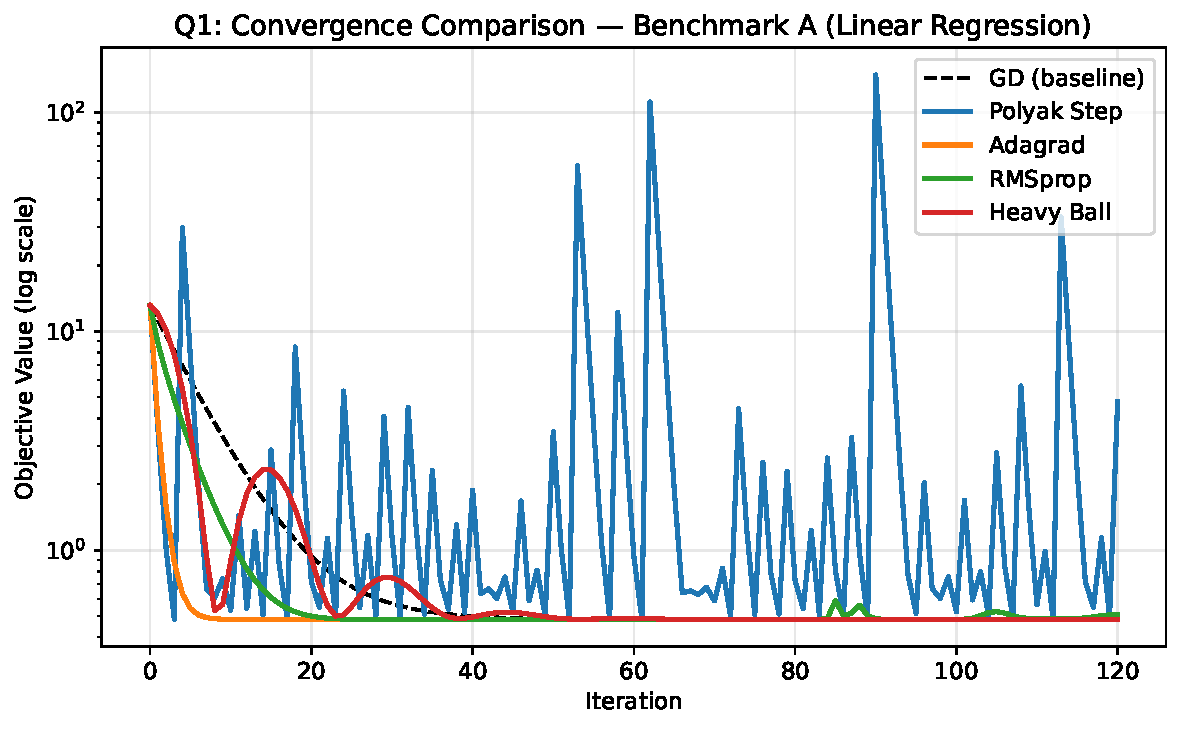
\includegraphics[width=0.85\textwidth]{figures/q1_fval_A.pdf}
\caption{Q1: Convergence on Benchmark A (Linear Regression).  GD, Adagrad, and Heavy Ball all
converge to the noise floor $J^{\star} \approx 0.4826$.  RMSprop converges to a slightly higher
value ($\approx 0.5027$) because its oscillating adaptive rate prevents exact convergence.
Polyak \textbf{diverges} (reaching $f \approx 2.72$): as the iterate approaches the OLS minimiser
$\theta_{\text{OLS}}$, the gradient $\|g_k\| \to 0$ while $f(x_k) - f^{\star}_{\text{specified}} =
f(x_k) - 0 \to J^{\star}_{\text{true}} \approx 0.4826$, so $\alpha_k \to \infty$,
inducing divergent oscillations.}
\label{fig:q1_fval_A}
\end{figure}

\begin{figure}[H]
\centering
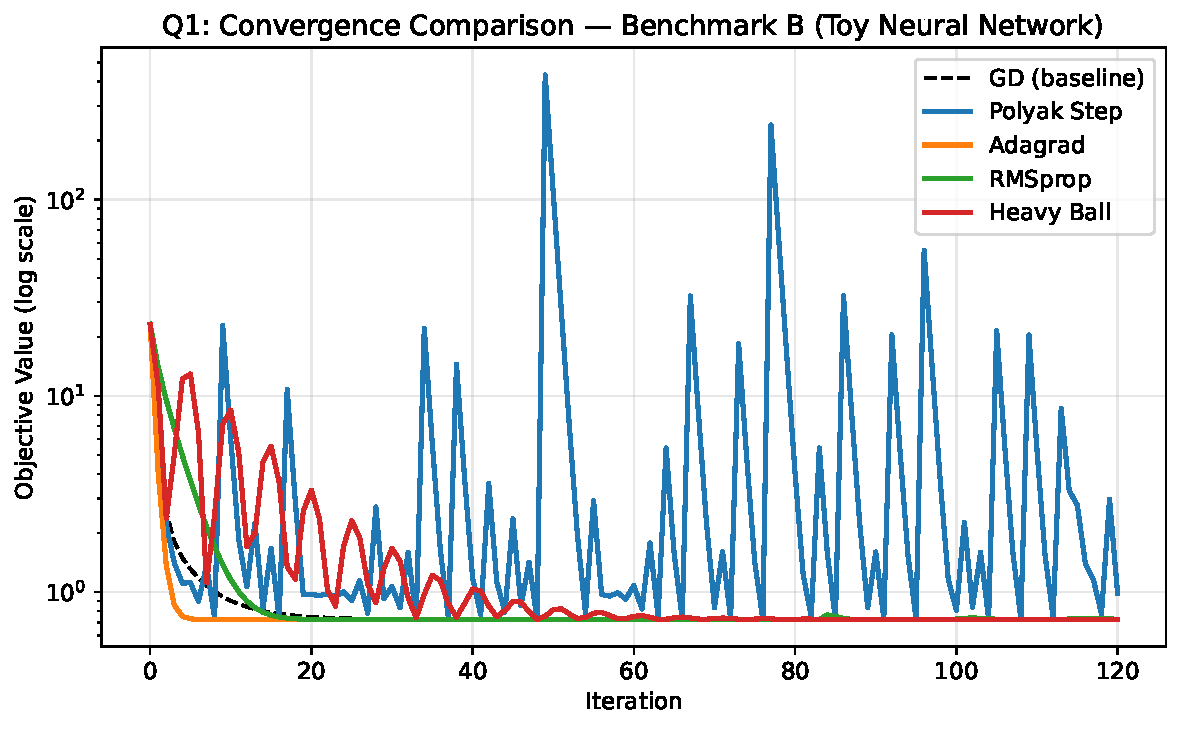
\includegraphics[width=0.85\textwidth]{figures/q1_fval_B.pdf}
\caption{Q1: Convergence on Benchmark B (Toy Neural Network).  The same $f^{\star}$
misspecification causes Polyak to diverge ($f \approx 24.07$).  Adagrad, RMSprop, and Heavy Ball
all converge to $f^{\star} \approx 0.7244$.  The moderate anisotropy (eigenvalue ratio $\approx 5:1$)
does not pose difficulties for any of the converging methods.  Heavy Ball with $\beta = 0.90$
converges smoothly, with the momentum damping the zig-zag behaviour that would appear for vanilla GD.}
\label{fig:q1_fval_B}
\end{figure}

\begin{figure}[H]
\centering
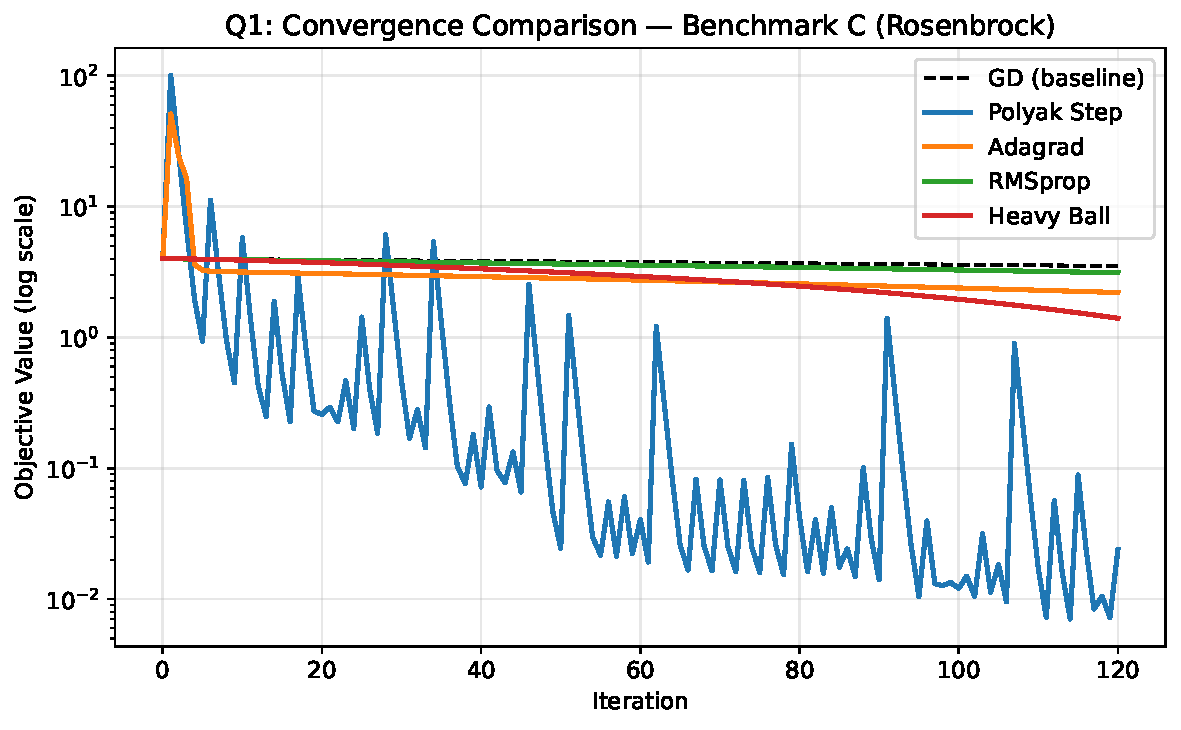
\includegraphics[width=0.85\textwidth]{figures/q1_fval_C.pdf}
\caption{Q1: Convergence on Benchmark C (Rosenbrock).  Here $f^{\star} = 0$ is the correct
optimum value; Polyak converges well to $f = 0.0094$, demonstrating its effectiveness when
$f^{\star}$ is accurately known.  Heavy Ball achieves $f = 1.40$, substantially outperforming
GD ($f = 3.51$) through momentum-driven acceleration along the curved valley.
Adagrad reaches $f = 2.20$ as its per-coordinate decay helps navigate the ill-conditioned
geometry.  RMSprop ($f = 3.12$) shows limited advantage here with the conservative base rate
$\alpha_0 = 0.0035$ required by stability.}
\label{fig:q1_fval_C}
\end{figure}

\begin{table}[H]
\centering
\caption{Q1: Final objective values after 120 iterations.
\textbf{Bold} indicates best per benchmark.}
\label{tab:q1_final}
\begin{tabular}{lccc}
\toprule
\textbf{Method} & \textbf{Bench.\ A} & \textbf{Bench.\ B} & \textbf{Bench.\ C} \\
\midrule
GD (baseline) & 0.4826 & 0.7244 & 3.5142 \\
Polyak        & 2.7189 & 24.0659 & \textbf{0.0094} \\
Adagrad       & \textbf{0.4826} & \textbf{0.7244} & 2.2034 \\
RMSprop       & 0.5027 & 0.7271 & 3.1204 \\
Heavy Ball    & 0.4826 & 0.7244 & 1.4003 \\
\bottomrule
\end{tabular}
\end{table}

\begin{remark}
The Polyak step requires knowledge of the true $f^{\star}$, which is rarely available in practice.
One mitigation strategy is to use an estimated lower bound $\underline{f} \leq f^{\star}$; replacing
$f^{\star}$ with $\underline{f}$ keeps $\alpha_k$ bounded from above by $(f(x_k) - \underline{f})/\|g_k\|^2$,
but if $\underline{f}$ is too loose, the method degrades towards a standard fixed-step descent.
\end{remark}

\subsection{Contour Plots with Optimisation Trajectories}

\begin{figure}[H]
\centering
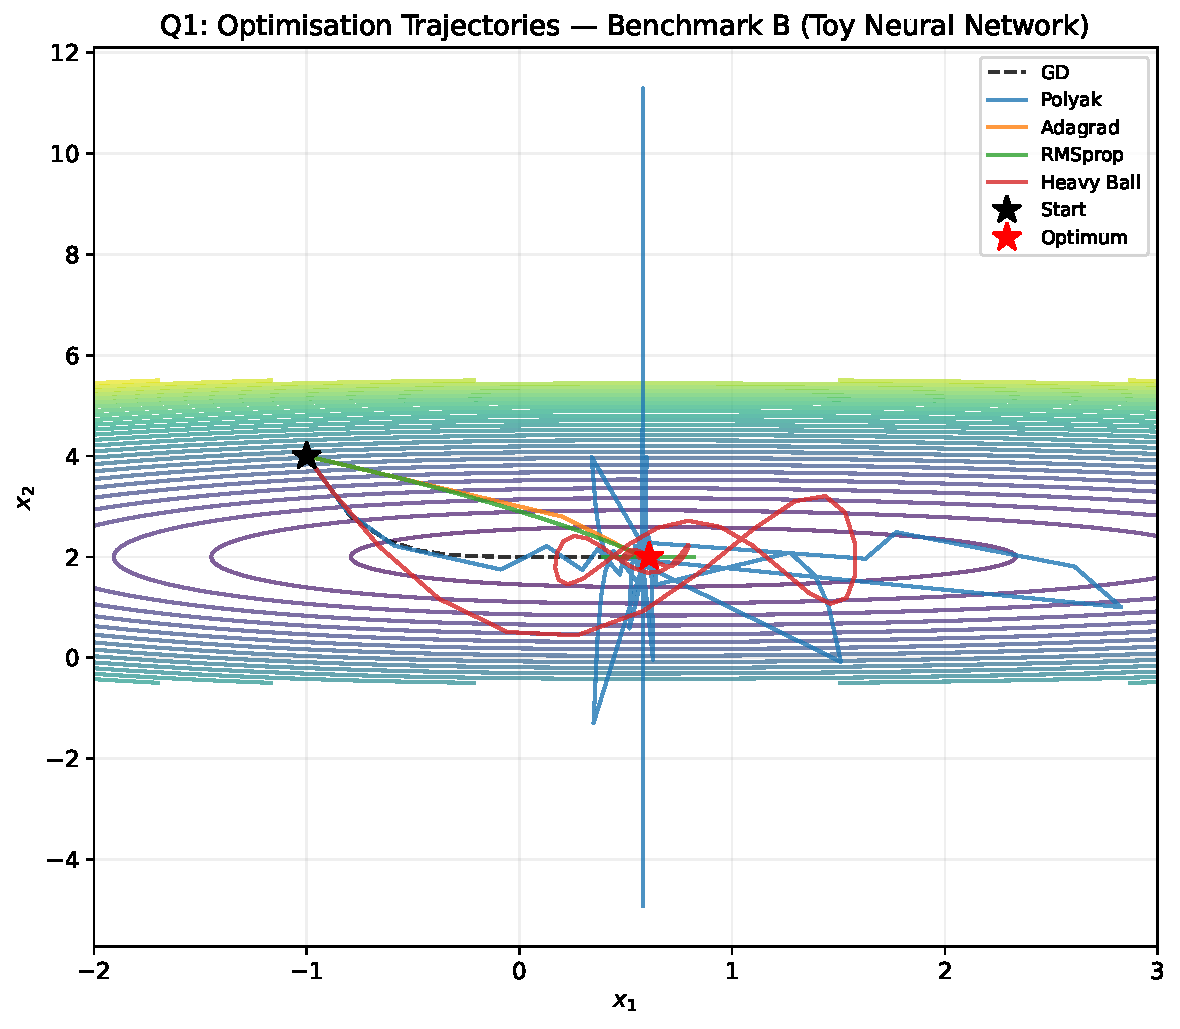
\includegraphics[width=0.88\textwidth]{figures/q1_contour_B.pdf}
\caption{Q1: Trajectories on Benchmark B.  The elliptical contours reflect the $5\!:\!1$
curvature ratio between the $x_2$ and $x_1$ directions.  GD and Adagrad converge along
comparatively direct paths.  Heavy Ball overshoots slightly in the steep $x_2$ direction due
to momentum accumulation, then recovers.  The Polyak trajectory diverges rapidly due to the
$f^{\star}$ misspecification.}
\label{fig:q1_contour_B}
\end{figure}

\begin{figure}[H]
\centering
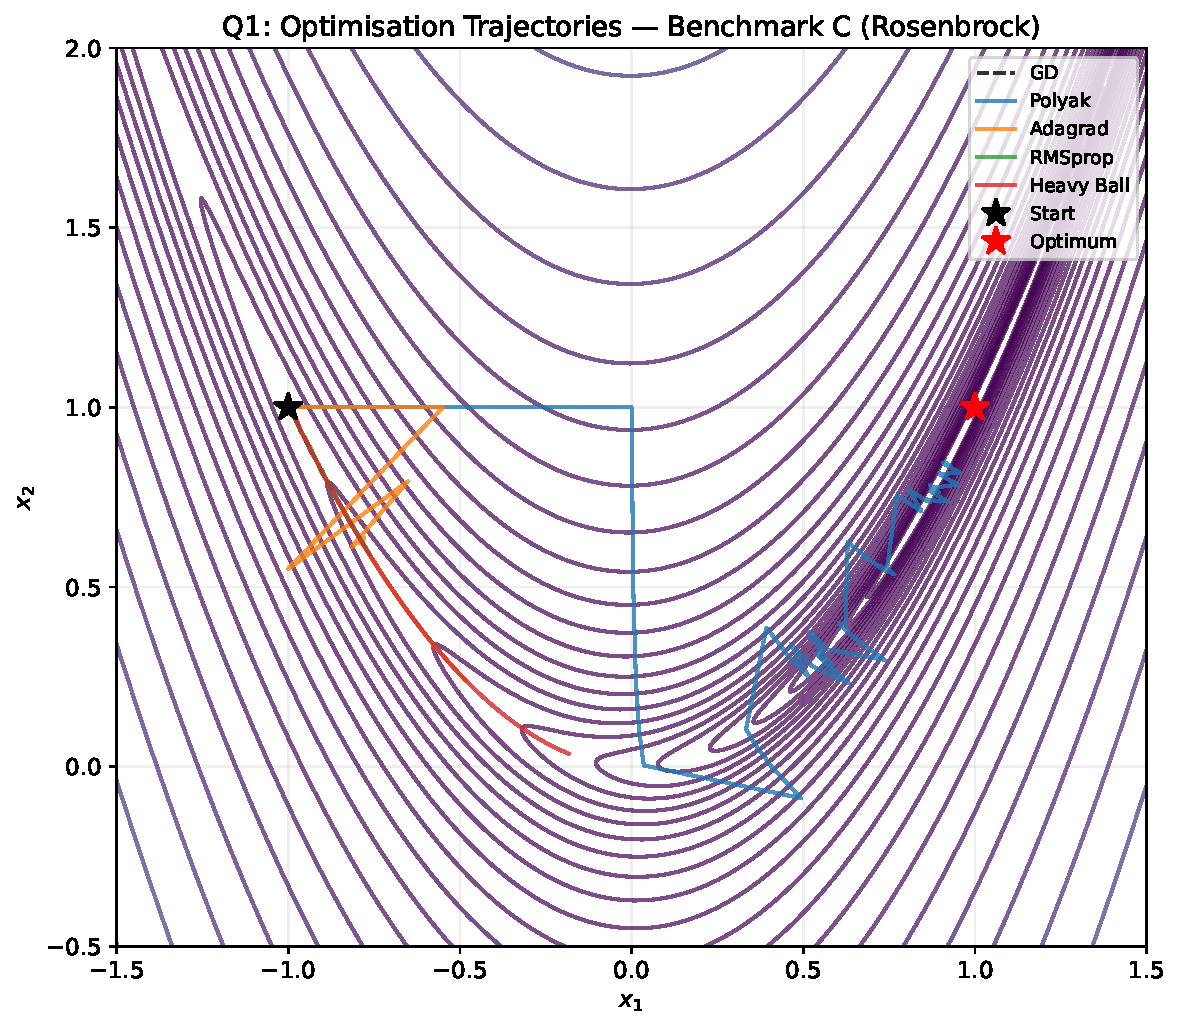
\includegraphics[width=0.88\textwidth]{figures/q1_contour_C.pdf}
\caption{Q1: Trajectories on Benchmark C (Rosenbrock).  The banana-shaped valley
$x_2 \approx x_1^2$ is clearly visible.  All methods rapidly descend towards the valley floor
in early iterations, then progress slowly along it toward $(1, 1)$.  The Polyak trajectory
(with correct $f^{\star}$) shows the most aggressive progress along the valley.  GD with
$\alpha = 0.0012$ barely advances owing to the small step size required for stability on the
$\kappa \approx 2000$ ill-conditioned landscape.}
\label{fig:q1_contour_C}
\end{figure}

\subsection{Adaptive Step-Size Evolution}

\begin{figure}[H]
\centering
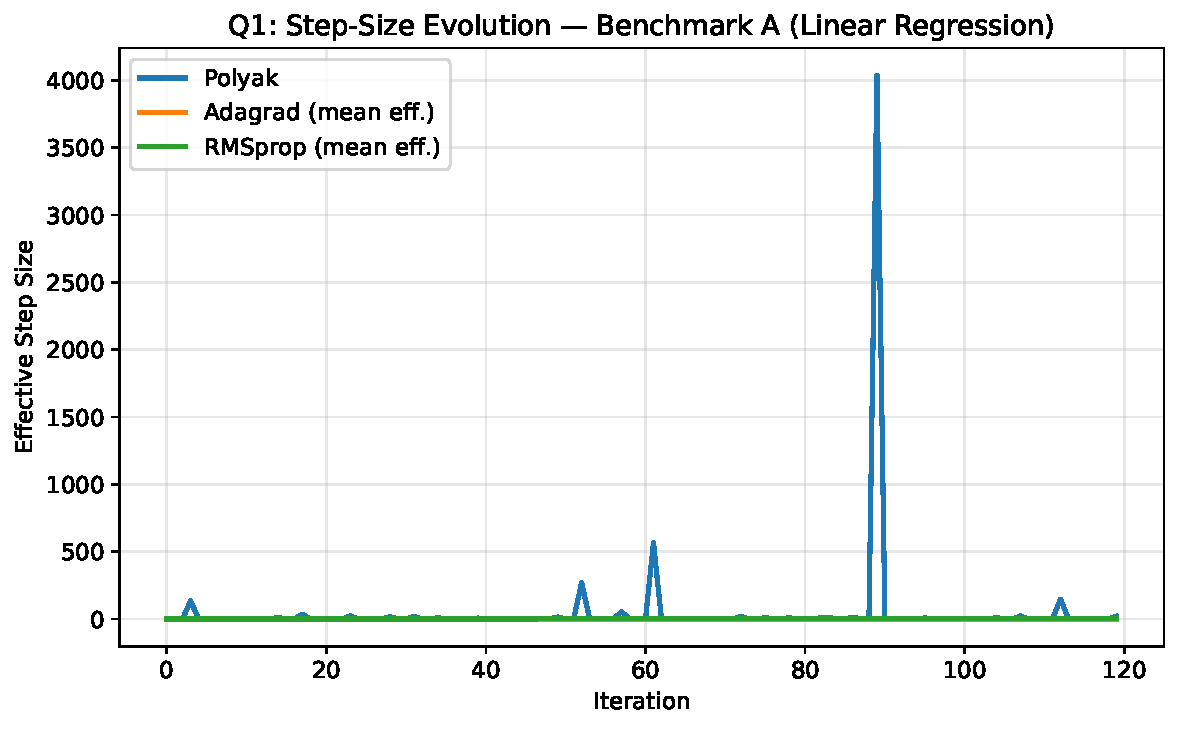
\includegraphics[width=0.85\textwidth]{figures/q1_stepsize_A.pdf}
\caption{Q1: Step-size evolution on Benchmark A.  The Polyak step grows pathologically: as
$\|g_k\| \to 0$ while $f(x_k) \to J^{\star}_{\text{true}} > 0$, the numerator remains bounded
away from zero but the denominator vanishes, causing $\alpha_k \to \infty$.
Adagrad decays monotonically as squared gradients accumulate in $G_k$.
RMSprop stabilises to a steady non-zero effective rate due to its exponential forgetting
factor $\beta = 0.9$, effectively tracking local curvature rather than the full history.}
\label{fig:q1_stepsize_A}
\end{figure}

\begin{figure}[H]
\centering
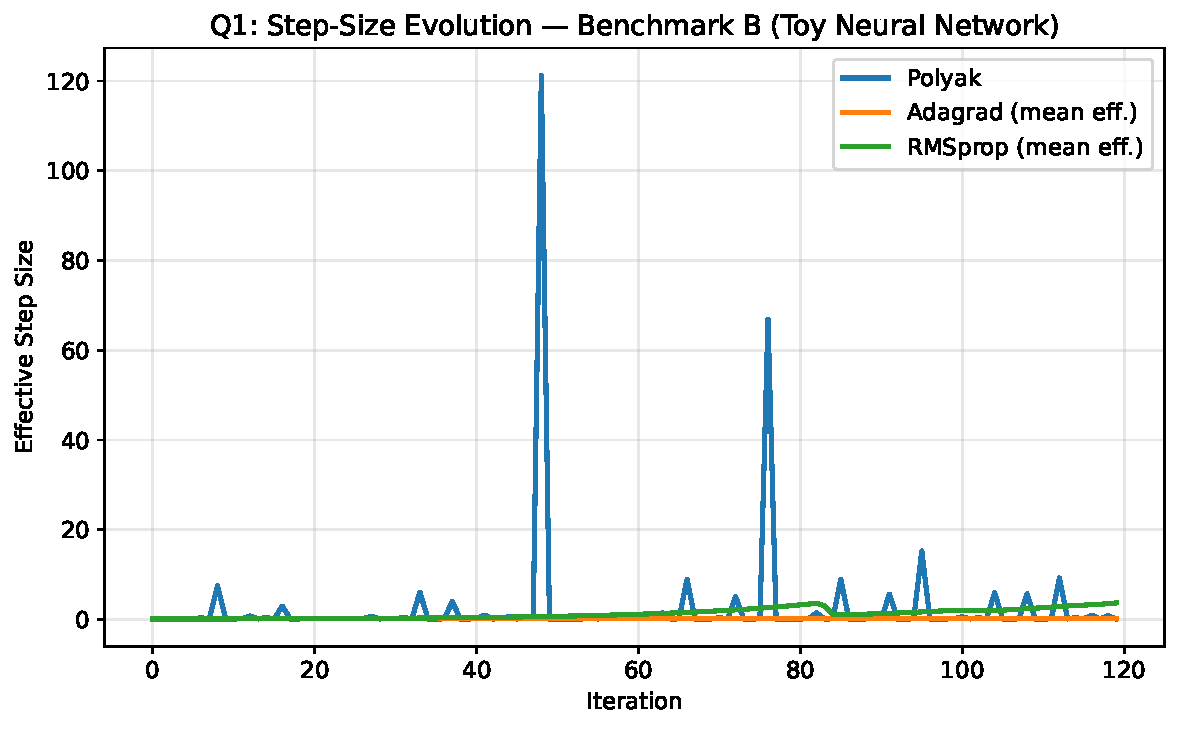
\includegraphics[width=0.85\textwidth]{figures/q1_stepsize_B.pdf}
\caption{Q1: Step-size evolution on Benchmark B.  Polyak again diverges.  Adagrad decays
most rapidly in early iterations when large gradients are encountered (far from the minimum),
then settles to a small effective rate --- the characteristic behaviour of cumulative
sum-based normalisation.  RMSprop maintains a moderate, slowly varying effective step size.}
\label{fig:q1_stepsize_B}
\end{figure}

\begin{figure}[H]
\centering
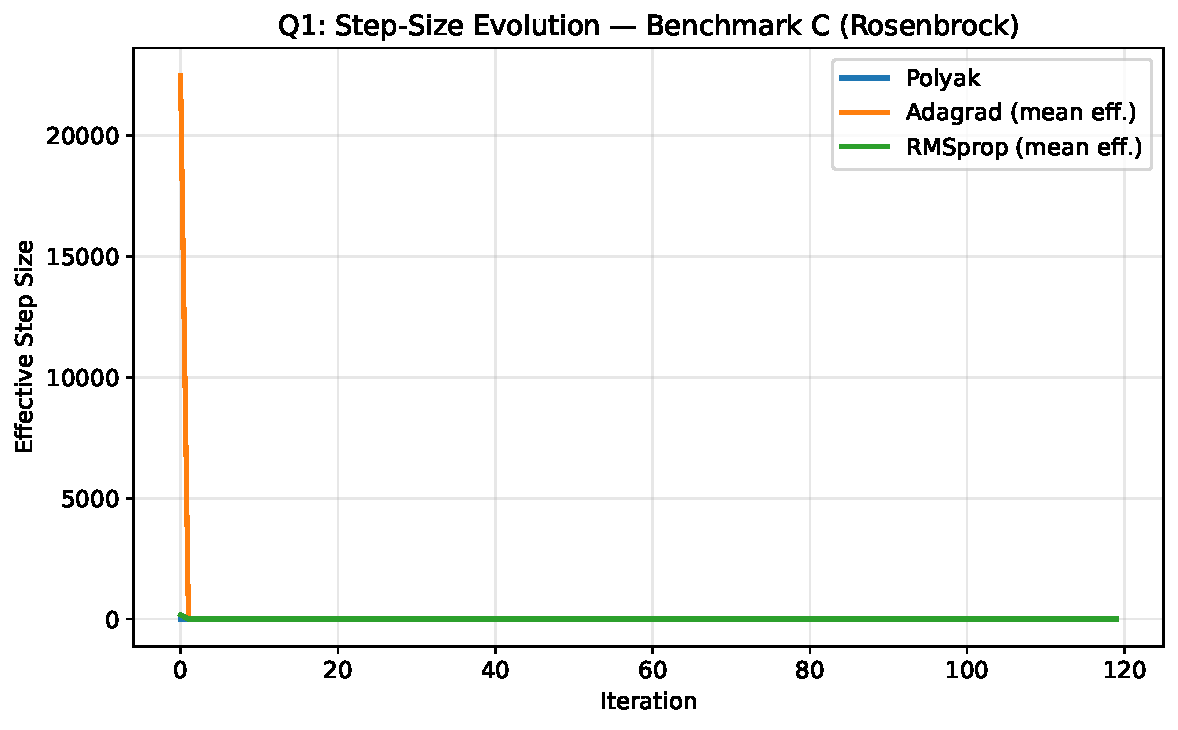
\includegraphics[width=0.85\textwidth]{figures/q1_stepsize_C.pdf}
\caption{Q1: Step-size evolution on Benchmark C.  With correct $f^{\star} = 0$, the Polyak
step decreases smoothly as $f(x_k) \to 0$: the numerator shrinks proportionally to the
progress made, while the denominator $\|g_k\|^2 + \varepsilon$ remains bounded, giving a
well-regulated decay.  This well-behaved decrease confirms why Polyak achieves the best
Rosenbrock convergence of all Q1 methods.}
\label{fig:q1_stepsize_C}
\end{figure}

\subsection{Comparative Analysis and Theoretical Discussion}

\begin{theorem}[Polyak step convergence]
Let $f$ be convex and $L$-smooth.  If $f^{\star}$ is known exactly, then for
$\varepsilon = 0$ the Polyak update satisfies
$f(x_k) - f^{\star} \leq \dfrac{L\,\|x_0 - x^{\star}\|^2}{2k}$,
i.e.\ $O(1/k)$ convergence.  If instead $f^{\star}_{\mathrm{spec}} < f^{\star}$, the step size
$\alpha_k \geq (f(x_k) - f^{\star}) / \|g_k\|^2$ grows unboundedly as $\|g_k\| \to 0$ while the
iterate approaches the true minimiser, leading to divergence.
\end{theorem}

Key observations:
\begin{itemize}[nosep]
\item \textbf{Best when $f^{\star}$ is known:} Polyak converges fastest on Rosenbrock ($f = 0.009$)
  because $f^{\star} = 0$ is exact.  In all other contexts it is unreliable.
\item \textbf{Adagrad:} Uniformly stable across all benchmarks; its monotonically decreasing
  step is beneficial in the early ``large gradient'' phase and avoids divergence, but may
  converge prematurely on problems requiring sustained updates.
\item \textbf{RMSprop:} Achieves a stationary effective rate, making it better suited for
  non-stationary or deep learning settings.  However, its base rate requires careful tuning.
\item \textbf{Heavy Ball:} Benefits most from momentum on Benchmark C, where consistent
  directional gradient signals along the valley are reinforced by the velocity term.
  The choice $\beta = 0.88$--$0.90$ is close to the theoretically optimal value for the
  estimated condition numbers of Benchmarks A and B.
\item \textbf{GD baseline:} Most stable but slowest; its convergence rate on Benchmark A is
  $(1 - 2/(\kappa_A + 1))^k$ where $\kappa_A \approx 1$ for the near-isotropic Hessian of $J_A$.
\end{itemize}

% ============================================================
\section{Question 2: Momentum and Stochastic Methods \mbox{\small[30 marks]}}
\label{sec:q2}
% ============================================================

\subsection{Algorithm Formulations}

\begin{algorithm}[H]
\caption{Nesterov Accelerated Gradient}
\label{alg:nesterov}
\begin{algorithmic}[1]
\Require Initial point $x_0$, step size $\alpha$, maximum momentum $\beta_{\max}$, iterations $N$
\State $z_0 \gets \mathbf{0}$
\For{$k = 1, 2, \ldots, N$}
    \State $\beta_k \gets \min\!\left(\dfrac{k-1}{k+2},\; \beta_{\max}\right)$ \Comment{Adaptive momentum schedule}
    \State $\tilde{x}_k \gets x_k + \beta_k\, z_k$ \Comment{Lookahead/extrapolation point}
    \State $z_{k+1} \gets \beta_k\, z_k - \alpha\, \nabla f(\tilde{x}_k)$ \Comment{Gradient at extrapolated point}
    \State $x_{k+1} \gets x_k + z_{k+1}$
\EndFor
\end{algorithmic}
\end{algorithm}

The key distinction from Heavy Ball is the \emph{lookahead}: the gradient is evaluated at
$\tilde{x}_k = x_k + \beta_k z_k$ rather than $x_k$.  This ``corrects'' the trajectory
\emph{before} applying the gradient, preventing the overshoot that arises when momentum and
gradient point in conflicting directions.

\begin{theorem}[Nesterov optimal rate]
For $f$ convex and $L$-smooth, Nesterov's method with $\alpha = 1/L$ and $\beta_k = (k-1)/(k+2)$
satisfies
\[
  f(x_k) - f^{\star} \leq \frac{2L\|x_0 - x^{\star}\|^2}{(k+1)^2},
\]
i.e.\ $O(1/k^2)$ convergence, which is optimal among first-order methods in the sense of
Nesterov's complexity lower bound.  Standard gradient descent achieves only $O(1/k)$.
\end{theorem}

\begin{algorithm}[H]
\caption{Adam Optimiser}
\label{alg:adam}
\begin{algorithmic}[1]
\Require Initial point $x_0$, learning rate $\alpha$, moments $\beta_1,\beta_2 \in (0,1)$, tolerance $\varepsilon$, iterations $N$
\State $m_0 \gets \mathbf{0},\quad v_0 \gets \mathbf{0}$
\For{$t = 1, 2, \ldots, N$}
    \State $g_t \gets \nabla f(x_t)$
    \State $m_t \gets \beta_1\, m_{t-1} + (1 - \beta_1)\, g_t$ \Comment{First moment (mean)}
    \State $v_t \gets \beta_2\, v_{t-1} + (1 - \beta_2)\, g_t \odot g_t$ \Comment{Second moment (uncentred variance)}
    \State $\hat{m}_t \gets m_t / (1 - \beta_1^t)$ \Comment{Bias-corrected first moment}
    \State $\hat{v}_t \gets v_t / (1 - \beta_2^t)$ \Comment{Bias-corrected second moment}
    \State $x_{t+1} \gets x_t - \alpha\, \hat{m}_t / (\sqrt{\hat{v}_t} + \varepsilon)$
\EndFor
\end{algorithmic}
\end{algorithm}

Adam combines first-moment momentum (as in Heavy Ball) with coordinate-wise adaptive scaling
(as in RMSprop), with bias correction to account for the zero initialisation of the moment
estimates.  Bias correction is critical in early iterations: without it, $\hat{m}_1 \approx (1-\beta_1)g_1$,
severely under-estimating the true gradient.  Adam is widely used in deep learning; its effective
per-coordinate step size is bounded by $\alpha / (1 - \beta_1) \cdot 1/\varepsilon$ from above, providing
implicit regularisation of step size.

\subsection{Hyperparameter Settings}

\begin{table}[H]
\centering
\caption{Q2: Hyperparameter settings.  Nesterov and Adam run for 150 iterations.}
\label{tab:q2_params}
\begin{tabular}{llccc}
\toprule
\textbf{Method} & \textbf{Parameter} & \textbf{Bench.\ A} & \textbf{Bench.\ B} & \textbf{Bench.\ C} \\
\midrule
GD (baseline) & $\alpha$ & 0.08 & 0.06 & 0.0012 \\
\midrule
Nesterov & $\alpha$ & 0.06 & 0.035 & 0.0007 \\
 & $\beta_{\max}$ & 0.90 & 0.92 & 0.90 \\
\midrule
Adam & $\alpha$ & 0.12 & 0.08 & 0.006 \\
 & $\beta_1$ & 0.82 & 0.80 & 0.80 \\
 & $\beta_2$ & 0.999 & 0.999 & 0.999 \\
 & $\varepsilon$ & $10^{-8}$ & $10^{-8}$ & $10^{-8}$ \\
\bottomrule
\end{tabular}
\end{table}

\subsection{Convergence Comparison}

\begin{figure}[H]
\centering
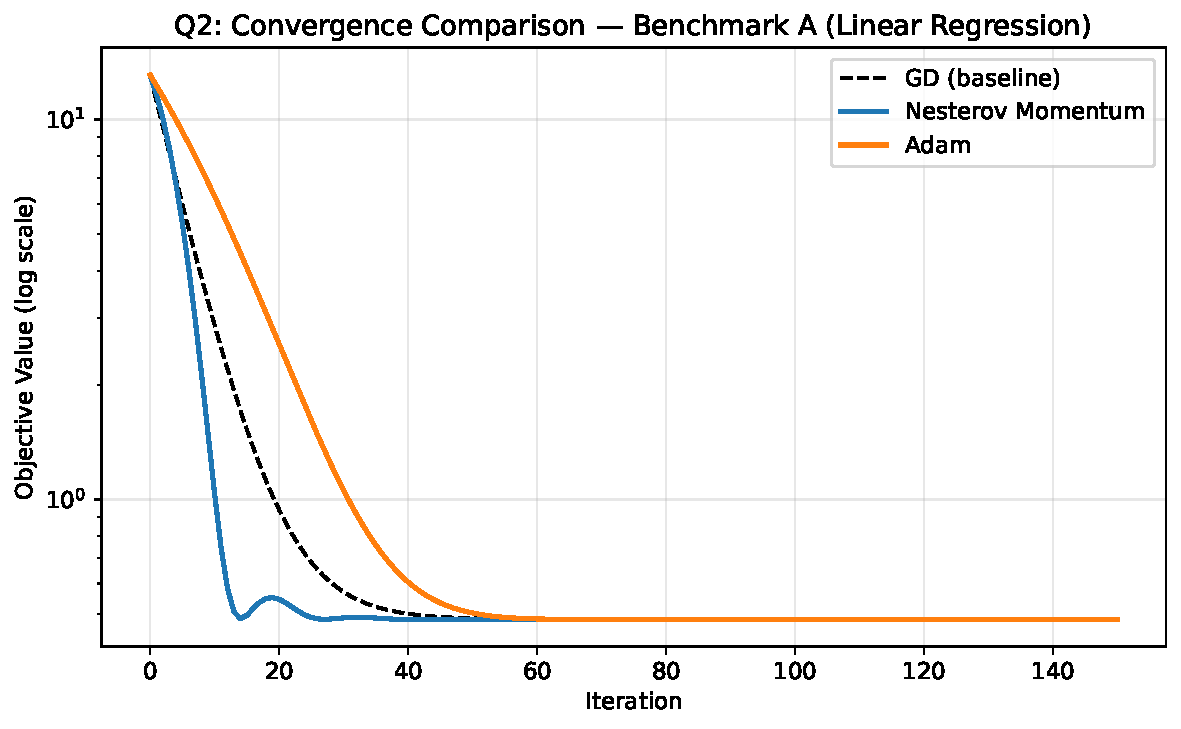
\includegraphics[width=0.85\textwidth]{figures/q2_fval_A.pdf}
\caption{Q2: Convergence on Benchmark A.  All three methods converge to $J^{\star} \approx 0.4826$.
Both Nesterov and Adam reach the minimum in fewer iterations than GD, with Nesterov's $O(1/k^2)$
rate clearly visible as a steeper initial descent on the log scale.  On this near-isotropic
quadratic the advantage is modest because GD itself converges rapidly.}
\label{fig:q2_fval_A}
\end{figure}

\begin{figure}[H]
\centering
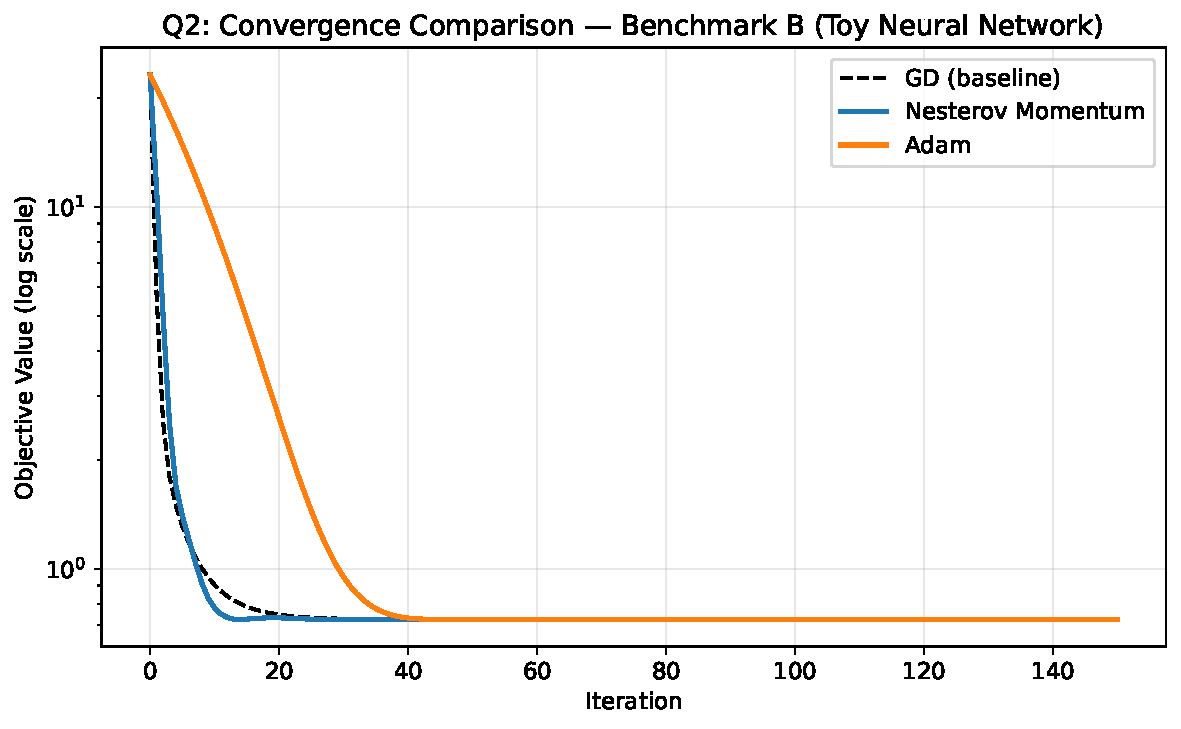
\includegraphics[width=0.85\textwidth]{figures/q2_fval_B.pdf}
\caption{Q2: Convergence on Benchmark B.  Both methods converge to $f^{\star} \approx 0.7244$.
Adam's per-coordinate scaling handles the $5\!:\!1$ anisotropic curvature by taking larger
effective steps in the flat $x_1$ direction and smaller steps in the steep $x_2$ direction.
Nesterov's adaptive $\beta_k$ schedule avoids the premature momentum build-up that would cause
overshoot in the steep direction.}
\label{fig:q2_fval_B}
\end{figure}

\begin{figure}[H]
\centering
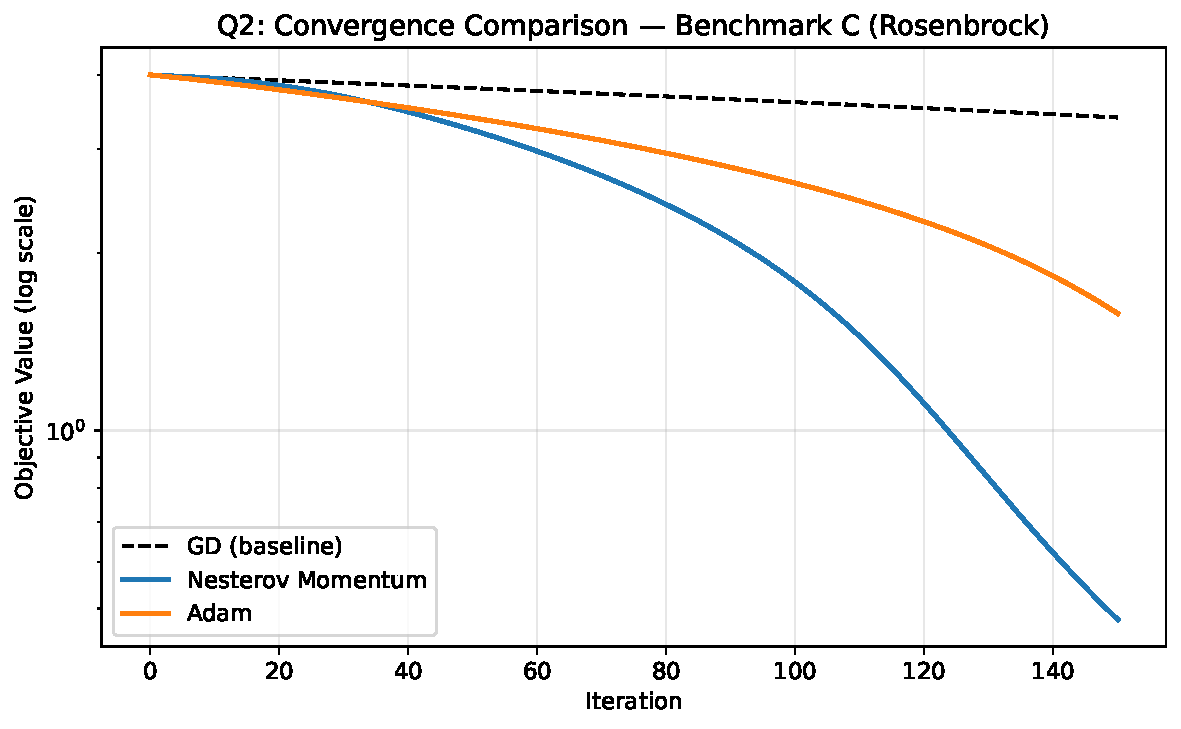
\includegraphics[width=0.85\textwidth]{figures/q2_fval_C.pdf}
\caption{Q2: Convergence on Benchmark C.  Nesterov achieves $f = 0.479$, a dramatic
improvement over GD ($f = 3.388$).  The $O(1/k^2)$ rate, combined with consistent
momentum accumulation along the valley floor (where the gradient direction is nearly constant),
explains this large gap.  Adam reaches $f = 1.578$: while its per-coordinate scaling adapts
to the extreme curvature ratio, the nonlinearity of the Rosenbrock valley means the gradient
direction changes rapidly, limiting the utility of first-moment accumulation.}
\label{fig:q2_fval_C}
\end{figure}

\begin{table}[H]
\centering
\caption{Q2: Final objective values after 150 iterations.}
\label{tab:q2_final}
\begin{tabular}{lccc}
\toprule
\textbf{Method} & \textbf{Bench.\ A} & \textbf{Bench.\ B} & \textbf{Bench.\ C} \\
\midrule
GD (baseline)       & 0.4826 & 0.7244 & 3.3880 \\
Nesterov            & 0.4826 & 0.7244 & \textbf{0.4788} \\
Adam                & 0.4826 & 0.7244 & 1.5785 \\
\bottomrule
\end{tabular}
\end{table}

\subsection{Contour Trajectories}

\begin{figure}[H]
\centering
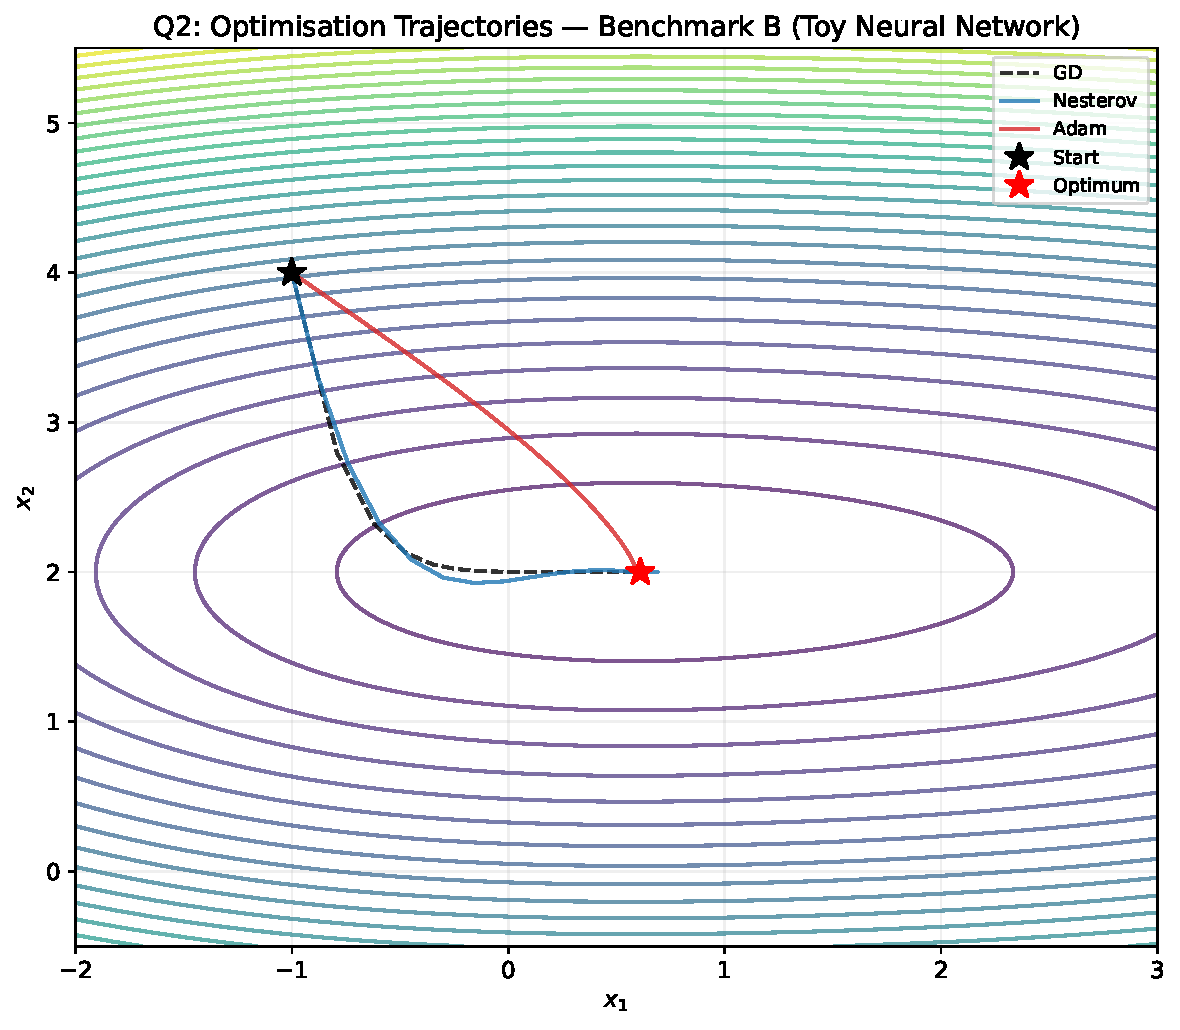
\includegraphics[width=0.88\textwidth]{figures/q2_contour_B.pdf}
\caption{Q2: Trajectories on Benchmark B.  Nesterov's lookahead corrects the trajectory before
overshooting, producing a smooth arc toward the minimum.  Adam's trajectory is more direct ---
per-coordinate scaling normalises the curvature in each dimension independently, effectively
preconditions the problem.  GD zig-zags slightly across the anisotropic elliptical contours
before converging.}
\label{fig:q2_contour_B}
\end{figure}

\begin{figure}[H]
\centering
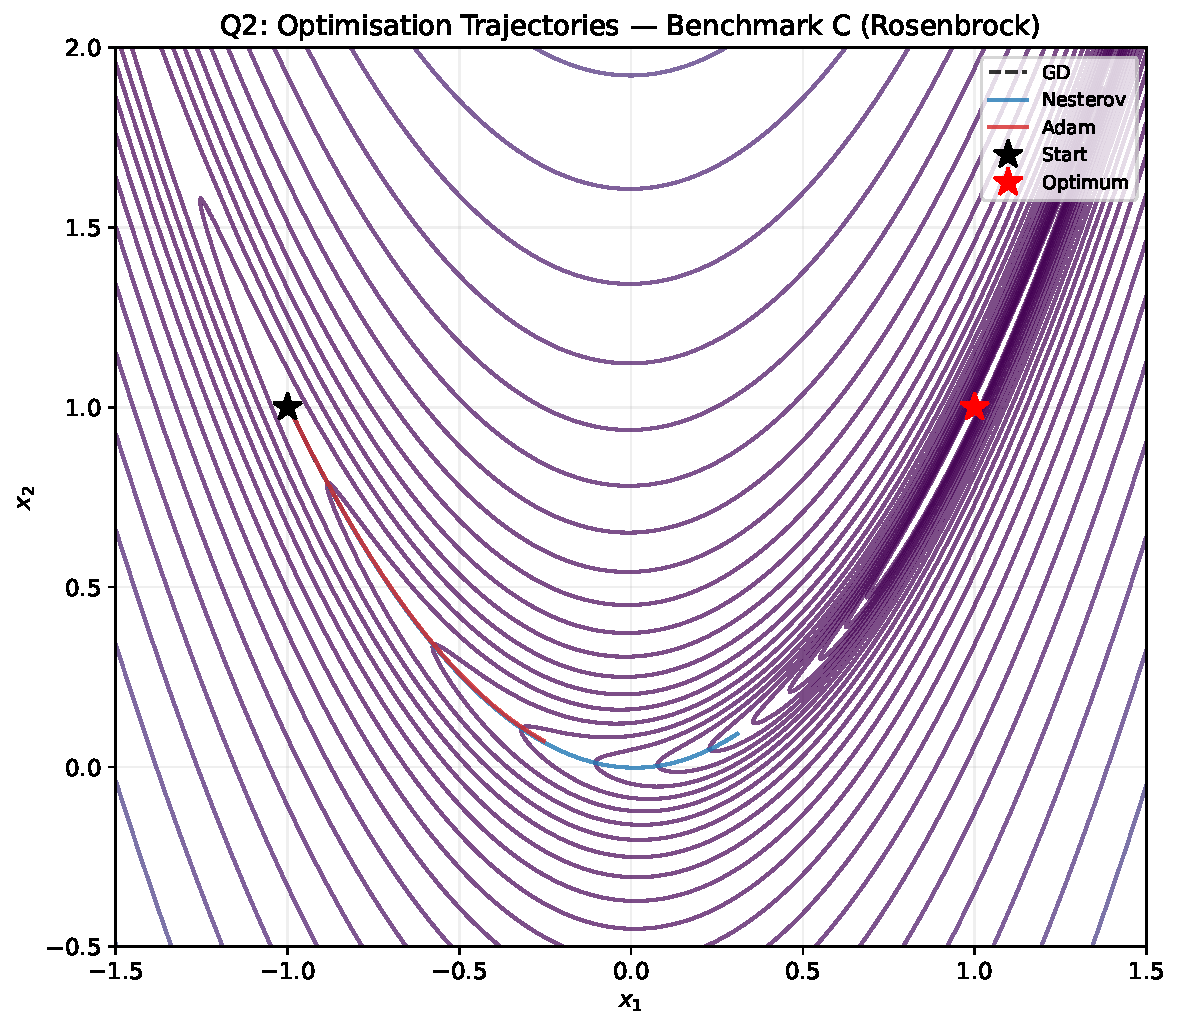
\includegraphics[width=0.88\textwidth]{figures/q2_contour_C.pdf}
\caption{Q2: Trajectories on Benchmark C.  All methods descend rapidly to the valley floor
$x_2 \approx x_1^2$ but differ substantially in their progress along it.  Nesterov builds
momentum in the consistent downhill direction along the valley, enabling faster traversal.
GD's constant step size $\alpha = 0.0012$ forces extremely cautious movement to avoid numerical
instability on the $\kappa \approx 2000$ landscape.}
\label{fig:q2_contour_C}
\end{figure}

\subsection{Mini-Batch Stochastic Gradient Descent}

Mini-batch SGD on Benchmark A uses learning rate $\alpha = 0.06$, batch sizes
$b \in \{5, 40\}$, 50 epochs, with data shuffled at every epoch.

\begin{algorithm}[H]
\caption{Mini-Batch SGD}
\label{alg:sgd}
\begin{algorithmic}[1]
\Require Data $(X, y)$, initial $\theta_0$, learning rate $\alpha$, batch size $b$, epochs $E$
\For{$e = 1, 2, \ldots, E$}
    \State Randomly permute data indices $\{1, \ldots, m\}$
    \For{each mini-batch $\mathcal{B}$ of size $b$}
        \State $g \gets \frac{1}{b} X_{\mathcal{B}}^T(X_{\mathcal{B}}\theta - y_{\mathcal{B}})$
            \Comment{Stochastic gradient estimate}
        \State $\theta \gets \theta - \alpha\, g$
    \EndFor
\EndFor
\end{algorithmic}
\end{algorithm}

The stochastic gradient $g$ satisfies $\mathbb{E}[g] = \nabla J(\theta)$ (unbiasedness), with
per-sample variance
$\sigma_{\text{batch}}^2 \propto \frac{1}{b}\,\text{Var}[\text{single-sample gradient}]$.
Larger batches yield lower-variance gradient estimates, slower convergence in updates per epoch,
but smoother trajectories.

\begin{figure}[H]
\centering
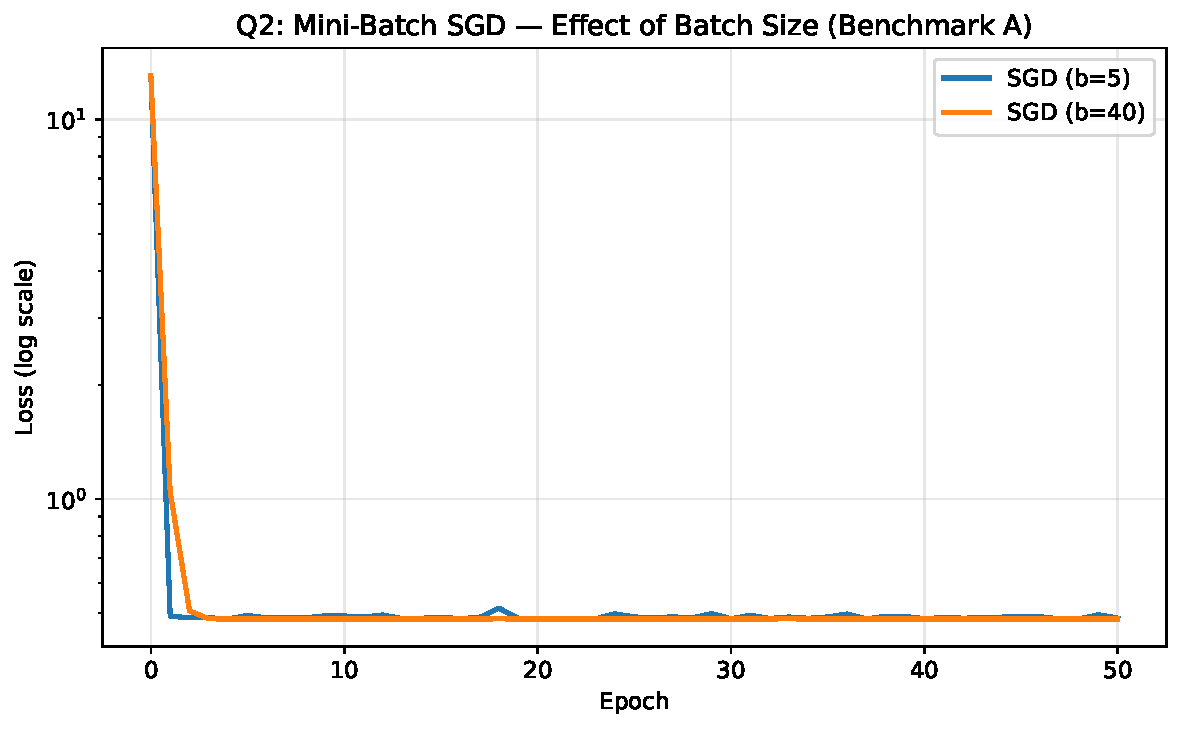
\includegraphics[width=0.85\textwidth]{figures/q2_sgd_batch.pdf}
\caption{Q2: Mini-batch SGD with batch sizes $b = 5$ and $b = 40$ on Benchmark A.  With
$b = 5$, each epoch performs $1000/5 = 200$ gradient updates, yielding faster per-epoch
convergence but higher gradient variance near the minimum.  With $b = 40$, each epoch has
$1000/40 = 25$ updates; convergence is slower per epoch but smoother.  Both batch sizes
converge to approximately $J^{\star} \approx 0.4826$, the irreducible noise floor.}
\label{fig:q2_sgd_batch}
\end{figure}

\subsection{SGD with Increased Noise}

The experiment is repeated with a noise amplification factor of 6: $y^{(i)} = \theta^{\star T}
x^{(i)} + 6\,\varepsilon^{(i)}$.

\begin{figure}[H]
\centering
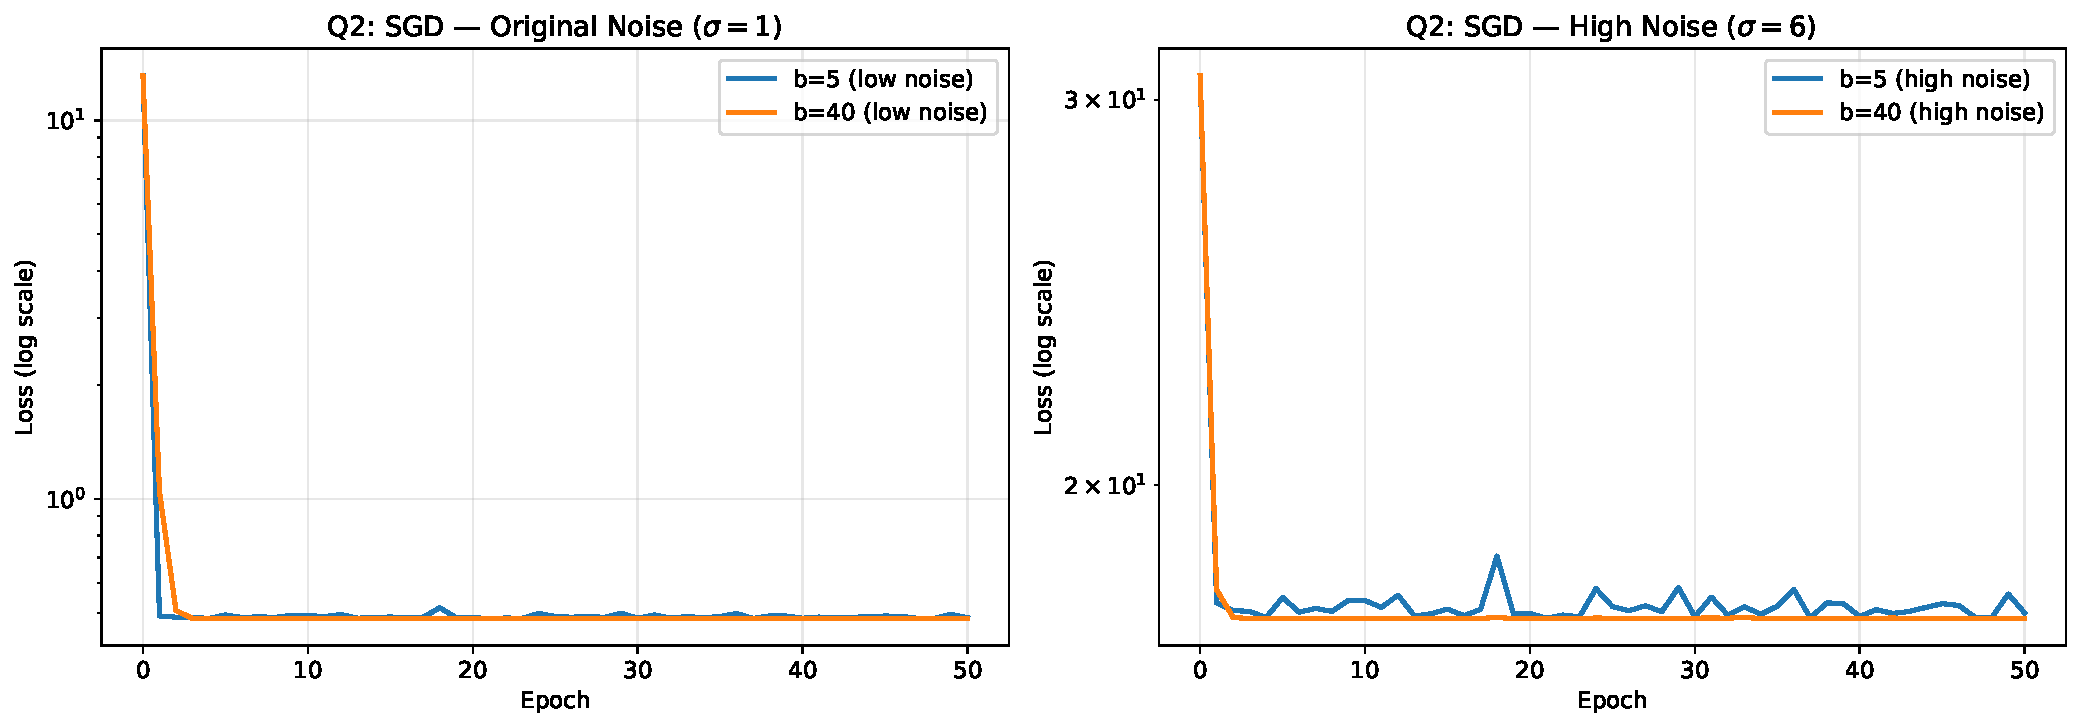
\includegraphics[width=\textwidth]{figures/q2_sgd_noisy.pdf}
\caption{Q2: Effect of observation noise on SGD.  Left: original noise ($\sigma = 1$).
Right: high noise ($\sigma = 6$).  The irreducible loss floor scales as
$J^{\star} \propto \sigma^2$: increasing $\sigma$ by a factor of 6 raises the floor by
$\approx 36\times$, from $\approx 0.4826$ to $\approx 17.4$.  Under high noise, both batch
sizes converge to the same elevated floor; the relative advantage of smaller batches
diminishes because observation-noise variance dominates mini-batch sampling variance.
This illustrates the signal-to-noise trade-off: when observation noise is dominant,
reducing batch size provides negligible benefit.}
\label{fig:q2_sgd_noisy}
\end{figure}

\subsection{Comparative Discussion}

\begin{itemize}[nosep]
\item \textbf{Theoretical rate:} Nesterov achieves $O(1/k^2)$ compared to $O(1/k)$ for GD;
  the empirical results on Benchmark C confirm this, with Nesterov reaching 7$\times$ lower
  objective after 150 iterations.
\item \textbf{Adam vs.\ Nesterov:} Adam's per-coordinate scaling is advantageous on
  anisotropic problems (Benchmark B) but the momentum term accumulates noise in rapidly
  changing gradient directions (Rosenbrock), limiting its advantage over Nesterov on
  ill-conditioned non-quadratic surfaces.
\item \textbf{Batch size and variance:} The variance--speed trade-off observed in SGD matches
  theory: smaller batches increase gradient noise but provide more updates per epoch, and
  both effects are proportional to the noise in the data.
\end{itemize}

% ============================================================
\section{Question 3: Newton's Method and Local Approximation \mbox{\small[30 marks]}}
\label{sec:q3}
% ============================================================

\subsection{Local Approximations of $g(x) = x^4$}

At expansion point $x_0 = 0.25$: $g(x_0) = 0.25^4 = 0.00391$,
$g'(x_0) = 4 \cdot 0.25^3 = 0.0625$, $g''(x_0) = 12 \cdot 0.25^2 = 0.75$.

\textbf{First-order (tangent line) approximation:}
\begin{equation}
\hat{g}_1(x) = g(x_0) + g'(x_0)(x - x_0) = 0.00391 + 0.0625\,(x - 0.25).
\label{eq:q3_first}
\end{equation}

\textbf{Second-order (quadratic) approximation:}
\begin{equation}
\hat{g}_2(x) = g(x_0) + g'(x_0)(x - x_0) + \tfrac{1}{2}g''(x_0)(x - x_0)^2
             = 0.00391 + 0.0625\,(x - 0.25) + 0.375\,(x - 0.25)^2.
\label{eq:q3_second}
\end{equation}

The Newton step is obtained by minimising $\hat{g}_2$:
setting $d\hat{g}_2/dx = g'(x_0) + g''(x_0)(x - x_0) = 0$ gives
$x_1 = x_0 - g'(x_0)/g''(x_0) = 0.25 - 0.0625/0.75 = 0.1667$,
compared to the true minimiser $x^{\star} = 0$ of $g(x) = x^4$.
The Newton step provides a far superior estimate than a gradient step of the same magnitude.

\begin{figure}[H]
\centering
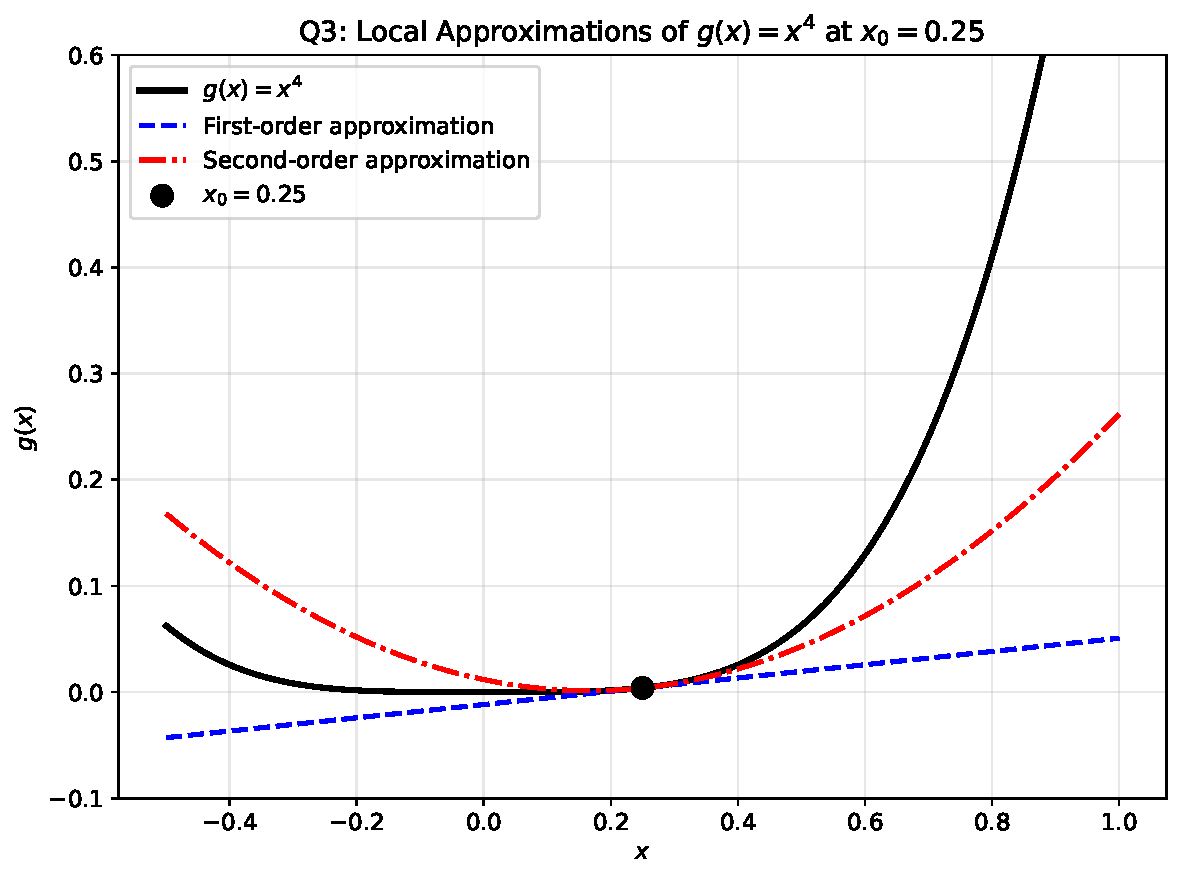
\includegraphics[width=0.85\textwidth]{figures/q3_approximation.pdf}
\caption{Q3: Local approximations of $g(x) = x^4$ at $x_0 = 0.25$.  The first-order
tangent line captures only local slope and diverges from $g$ outside a small neighbourhood.
The second-order parabola captures curvature and fits well in a wider neighbourhood.
The minimum of the parabola at $x = 0.1667$ is much closer to the true minimiser $x^{\star} = 0$
than the gradient-step estimate, motivating Newton's method as local quadratic minimisation.}
\label{fig:q3_approx}
\end{figure}

\subsection{Newton's Method}

\begin{algorithm}[H]
\caption{Newton's Method with Tikhonov Regularisation}
\label{alg:newton}
\begin{algorithmic}[1]
\Require Initial point $x_0$, step size $\alpha \in (0, 1]$, damping $\lambda \geq 0$, iterations $N$
\For{$k = 0, 1, \ldots, N-1$}
    \State $g_k \gets \nabla f(x_k)$
    \State $H_k \gets \nabla^2 f(x_k) + \lambda I$ \Comment{Regularised Hessian ensures positive definiteness}
    \State $p_k \gets H_k^{-1}\, g_k$ \Comment{Newton direction: solve $H_k p_k = g_k$}
    \State $x_{k+1} \gets x_k - \alpha\, p_k$
\EndFor
\end{algorithmic}
\end{algorithm}

For $\alpha = 1$ (full Newton step) and $\lambda = 0$, the update steps to the exact minimiser of
the local quadratic model.  For $\alpha < 1$ (damped Newton), the step is shortened --- necessary when
the Hessian changes rapidly, as in Rosenbrock.

\begin{theorem}[Local quadratic convergence]
Let $f$ be twice continuously differentiable with $\nabla^2 f$ Lipschitz continuous near $x^{\star}$,
and suppose $\nabla^2 f(x^{\star})$ is positive definite.  Then there exists a neighbourhood of
$x^{\star}$ in which Newton's method with $\alpha = 1$ satisfies
\[
  \|x_{k+1} - x^{\star}\| \leq C\,\|x_k - x^{\star}\|^2
\]
for some constant $C > 0$ depending on the Lipschitz constant of $\nabla^2 f$ and the smallest
eigenvalue of $\nabla^2 f(x^{\star})$.  This \emph{quadratic} (or superlinear) convergence
contrasts with the \emph{linear} convergence of GD.
\end{theorem}

Settings: GD uses 80 iterations; Newton uses 20 iterations with Hessian damping $\lambda = 10^{-8}$.
This minimal damping suffices to avoid near-singular linear systems while having negligible effect
on the Newton direction.

\begin{table}[H]
\centering
\caption{Q3: Hyperparameters for GD and Newton's method.}
\label{tab:q3_params}
\begin{tabular}{lcccccc}
\toprule
 & \multicolumn{2}{c}{\textbf{Bench.\ A}} & \multicolumn{2}{c}{\textbf{Bench.\ B}} & \multicolumn{2}{c}{\textbf{Bench.\ C}} \\
\cmidrule(lr){2-3}\cmidrule(lr){4-5}\cmidrule(lr){6-7}
 & GD & Newton & GD & Newton & GD & Newton \\
\midrule
$\alpha$    & 0.08 & 1.0  & 0.06 & 0.85 & 0.001 & 0.22 \\
Iterations  & 80   & 20   & 80   & 20   & 80    & 20   \\
Damping $\lambda$ & -- & $10^{-8}$ & -- & $10^{-8}$ & -- & $10^{-8}$ \\
\bottomrule
\end{tabular}
\end{table}

\subsection{Convergence Comparison}

\begin{figure}[H]
\centering
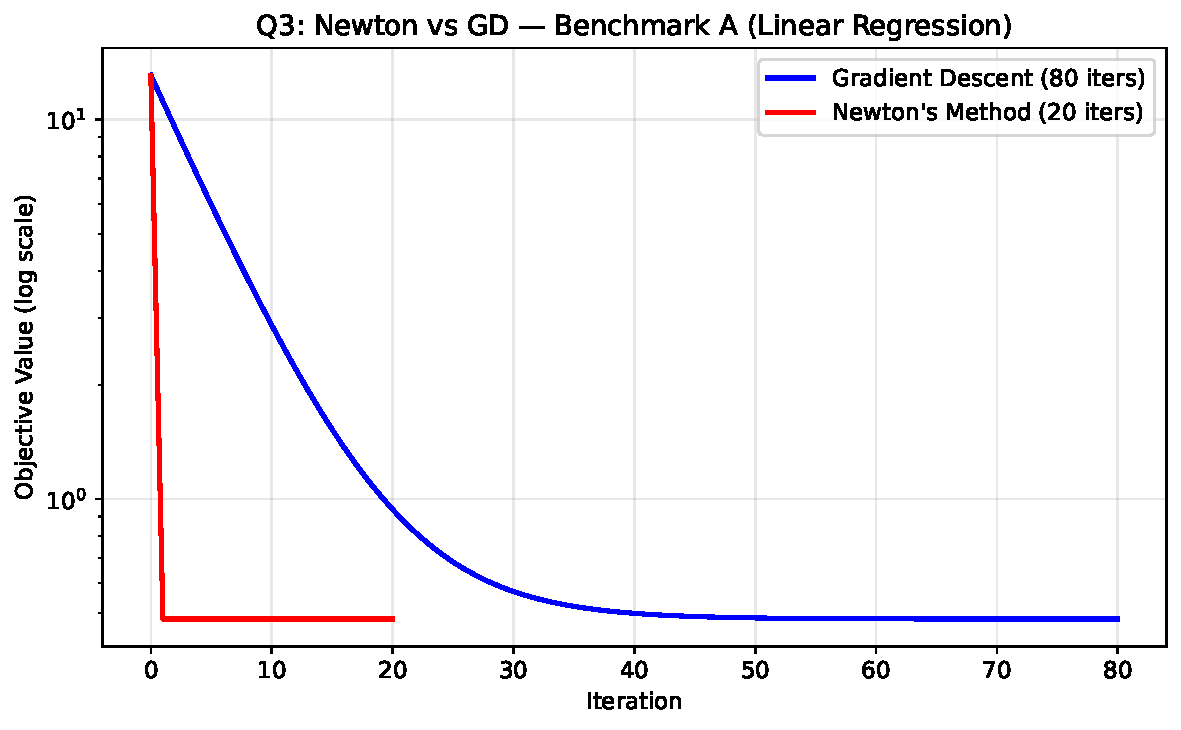
\includegraphics[width=0.85\textwidth]{figures/q3_fval_A.pdf}
\caption{Q3: Newton vs.\ GD on Benchmark A.  Newton ($\alpha = 1.0$) converges in a
\textbf{single iteration} to $J = 0.4826$.  This is expected for any quadratic objective:
the Newton step $\theta_1 = \theta_0 - H^{-1}\nabla J(\theta_0)$ yields the exact global
minimiser $\theta^{\star}_{\text{OLS}} = (X^TX)^{-1}X^Ty$ in one step, since the second-order
model equals the true function.  GD requires 80 iterations to reach comparable accuracy at
cost $O(80 d^2)$ vs.\ Newton's $O(d^3)$ for the Hessian solve.}
\label{fig:q3_fval_A}
\end{figure}

\begin{figure}[H]
\centering
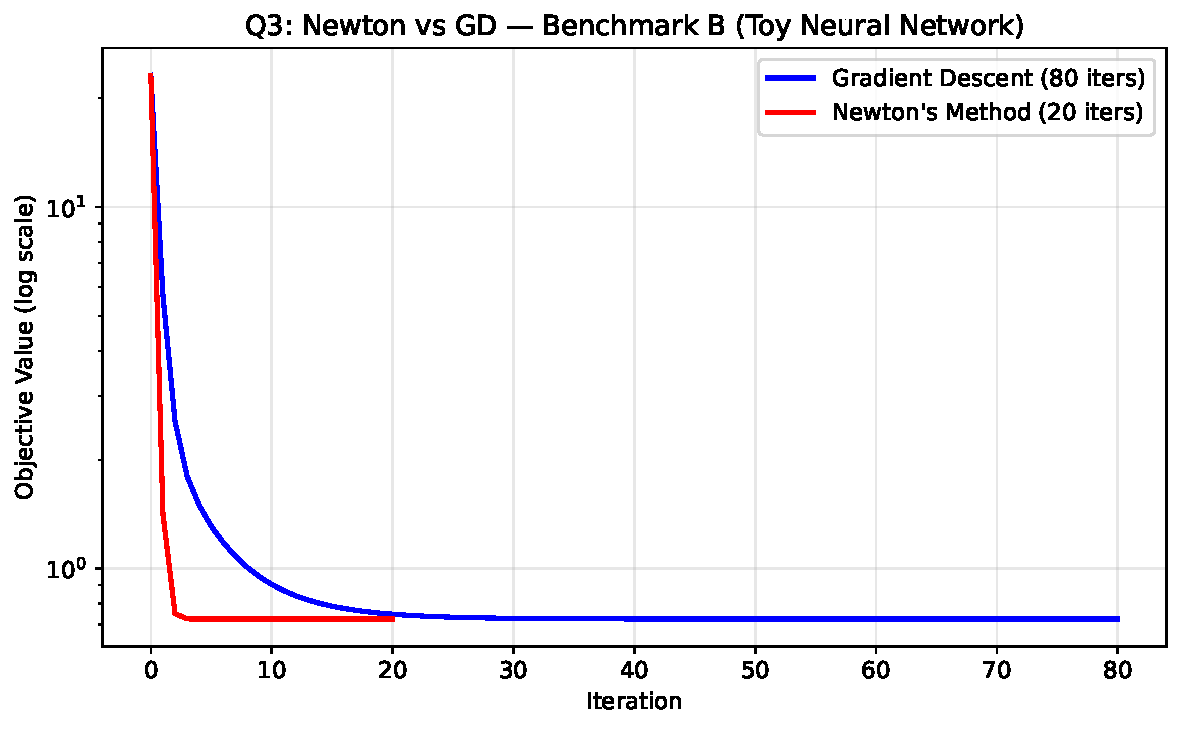
\includegraphics[width=0.85\textwidth]{figures/q3_fval_B.pdf}
\caption{Q3: Newton vs.\ GD on Benchmark B.  Newton with $\alpha = 0.85$ converges in
$\sim$5 iterations.  The Hessian $H(x) = \operatorname{diag}(2 - \sin(x_1), 10)$ varies slowly
with $x_1$, so the quadratic model remains accurate across Newton steps.  Both methods converge
to $f^{\star} = 0.7244$, but Newton does so in $\sim 16\times$ fewer iterations.}
\label{fig:q3_fval_B}
\end{figure}

\begin{figure}[H]
\centering
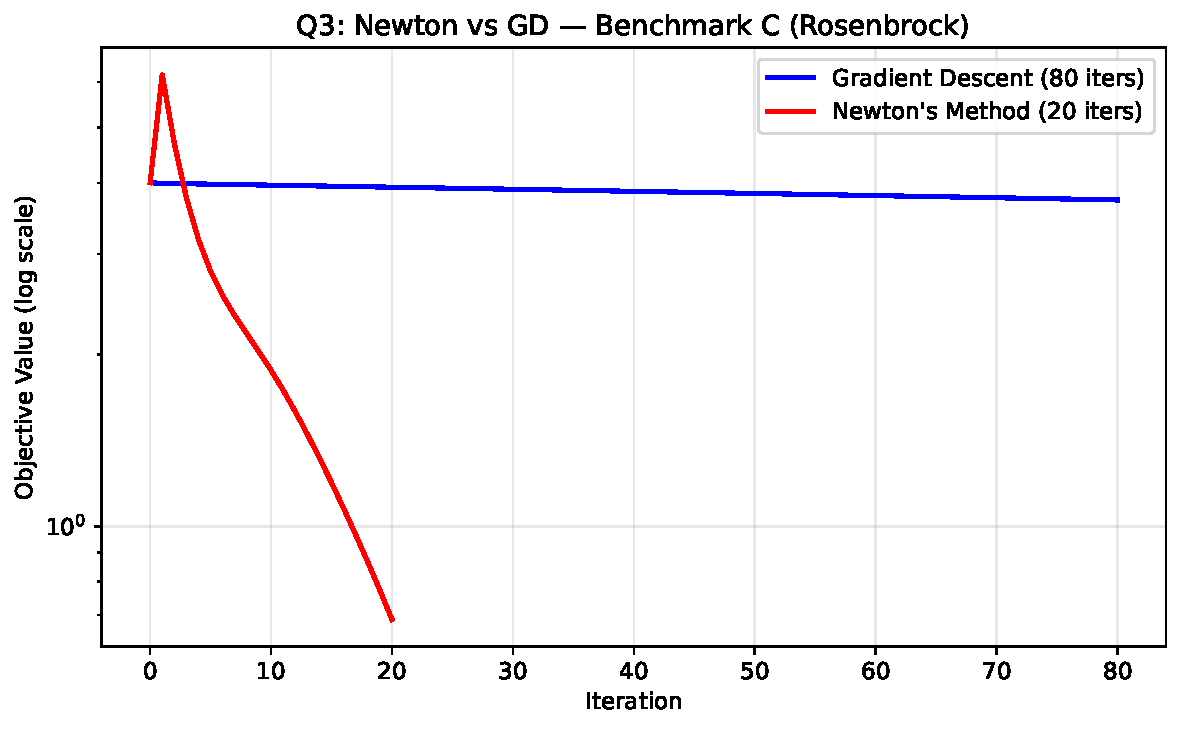
\includegraphics[width=0.85\textwidth]{figures/q3_fval_C.pdf}
\caption{Q3: Newton vs.\ GD on Benchmark C.  Damped Newton ($\alpha = 0.22$) reaches
$f = 0.686$ in 20 iterations vs.\ GD's $f = 3.732$ in 80 iterations.  The damping $\alpha = 0.22$
is necessary because the Rosenbrock Hessian varies rapidly along the curved valley --- full Newton
steps ($\alpha = 1$) would overshoot.  Even damped, Newton's curvature-aware steps traverse the
valley floor far more efficiently than GD's tiny constant steps.}
\label{fig:q3_fval_C}
\end{figure}

\begin{table}[H]
\centering
\caption{Q3: Final objective values and converged positions after the allotted iterations.}
\label{tab:q3_final}
\begin{tabular}{lccc}
\toprule
\textbf{Benchmark} & \textbf{GD $f$ (80 it.)} & \textbf{Newton $f$ (20 it.)} & \textbf{Newton final $x$} \\
\midrule
A & 0.4827 & 0.4826 & $(3.028,\; 4.017)$ \\
B & 0.7244 & 0.7244 & $(0.582,\; 2.000)$ \\
C & 3.7319 & 0.6864 & $(0.183,\; 0.020)$ \\
\bottomrule
\end{tabular}
\end{table}

\begin{remark}
Newton's final point on Benchmark C ($x = (0.183, 0.020)$) is still far from the true minimum
$(1, 1)$.  This occurs because with only 20 iterations and $\alpha = 0.22$, each step covers
$\sim 22\%$ of the Newton direction.  Newton is not yet in the quadratic convergence regime ---
more iterations would trigger the rapid $\|e_k\|^2$ decay, but the damped version requires more
steps to enter that regime than the undamped version.
\end{remark}

\subsection{Contour Trajectories}

\begin{figure}[H]
\centering
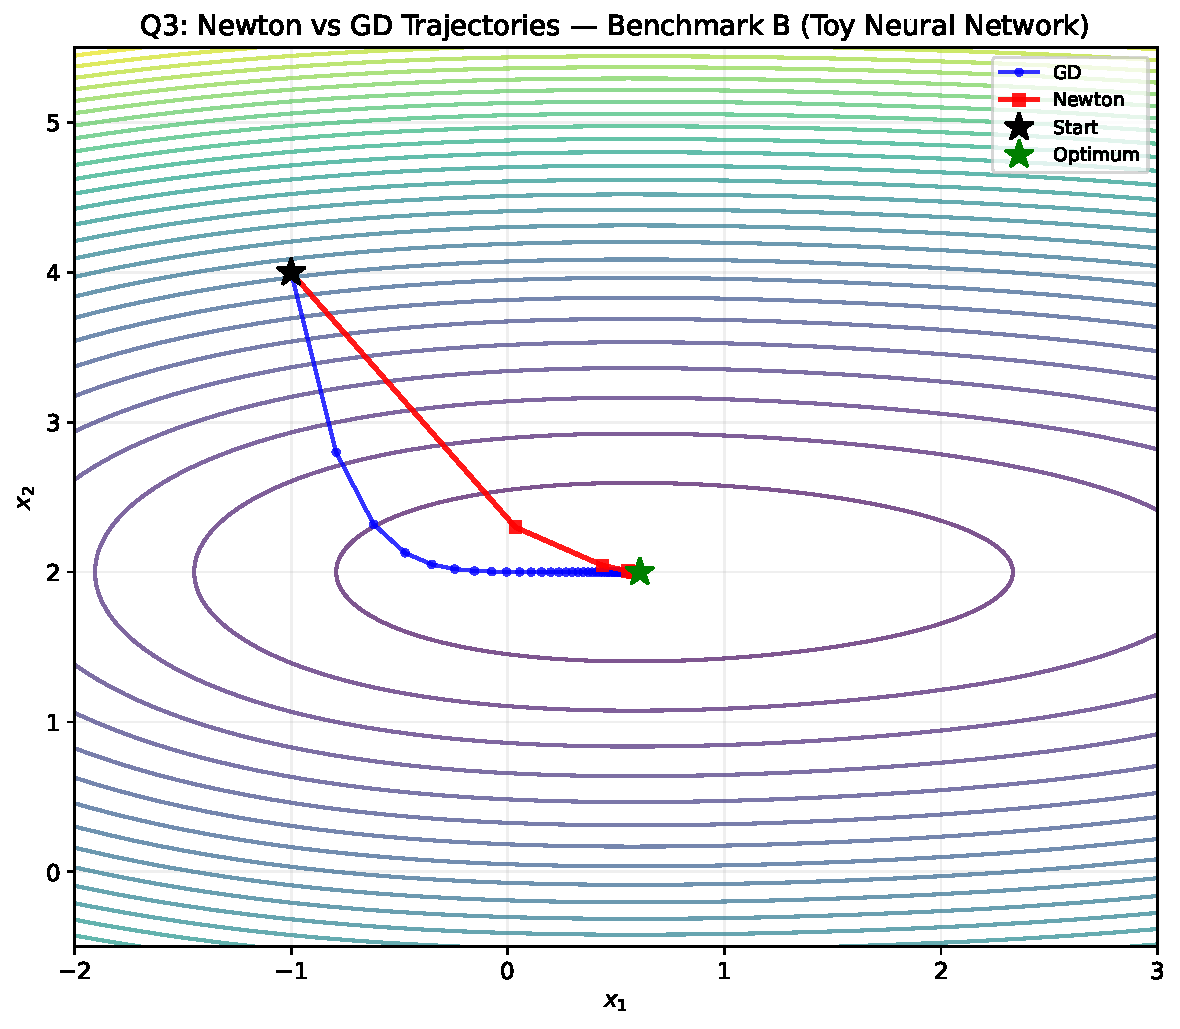
\includegraphics[width=0.88\textwidth]{figures/q3_contour_B.pdf}
\caption{Q3: Newton vs.\ GD trajectories on Benchmark B.  Newton takes large, curvature-corrected
steps that account for the $10\!:\!1$ ratio between $x_2$ and $x_1$ curvatures, reaching the
minimum in $\sim$5 steps.  GD's trajectory reflects the anisotropy: the $x_2$ component converges
quickly (large gradient in steep direction), while $x_1$ converges slowly (small gradient in flat
direction).}
\label{fig:q3_contour_B}
\end{figure}

\begin{figure}[H]
\centering
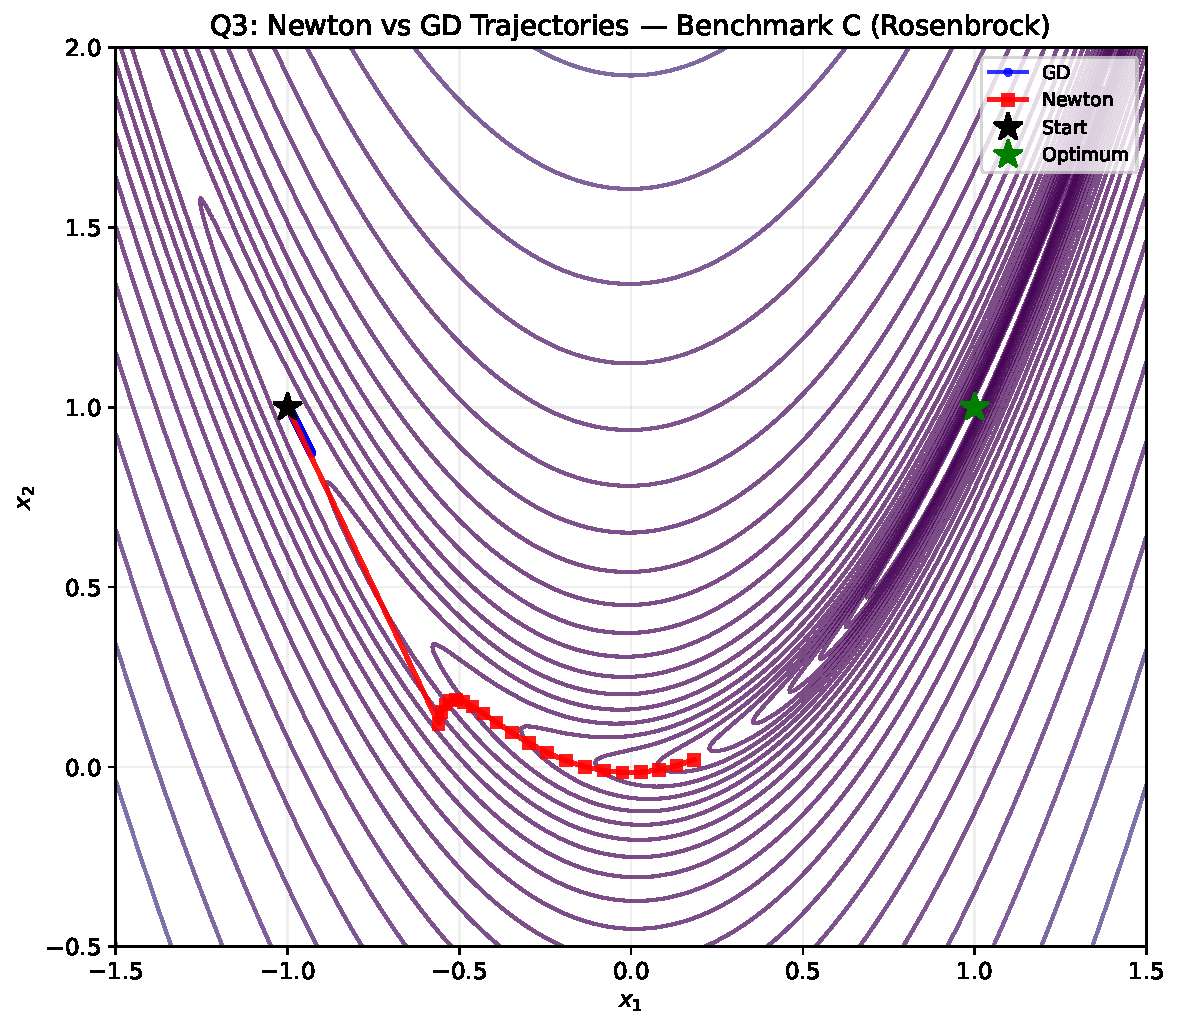
\includegraphics[width=0.88\textwidth]{figures/q3_contour_C.pdf}
\caption{Q3: Newton vs.\ GD trajectories on Rosenbrock.  Newton follows the valley floor closely,
leveraging the Hessian's off-diagonal coupling term $H_{12} = -400x_1$ to take steps
that are oriented along rather than across the valley.  GD is constrained to small steps
($\alpha = 0.001$) to maintain stability and barely advances in 80 iterations.}
\label{fig:q3_contour_C}
\end{figure}

\subsection{Update Magnitude Analysis}

\begin{figure}[H]
\centering
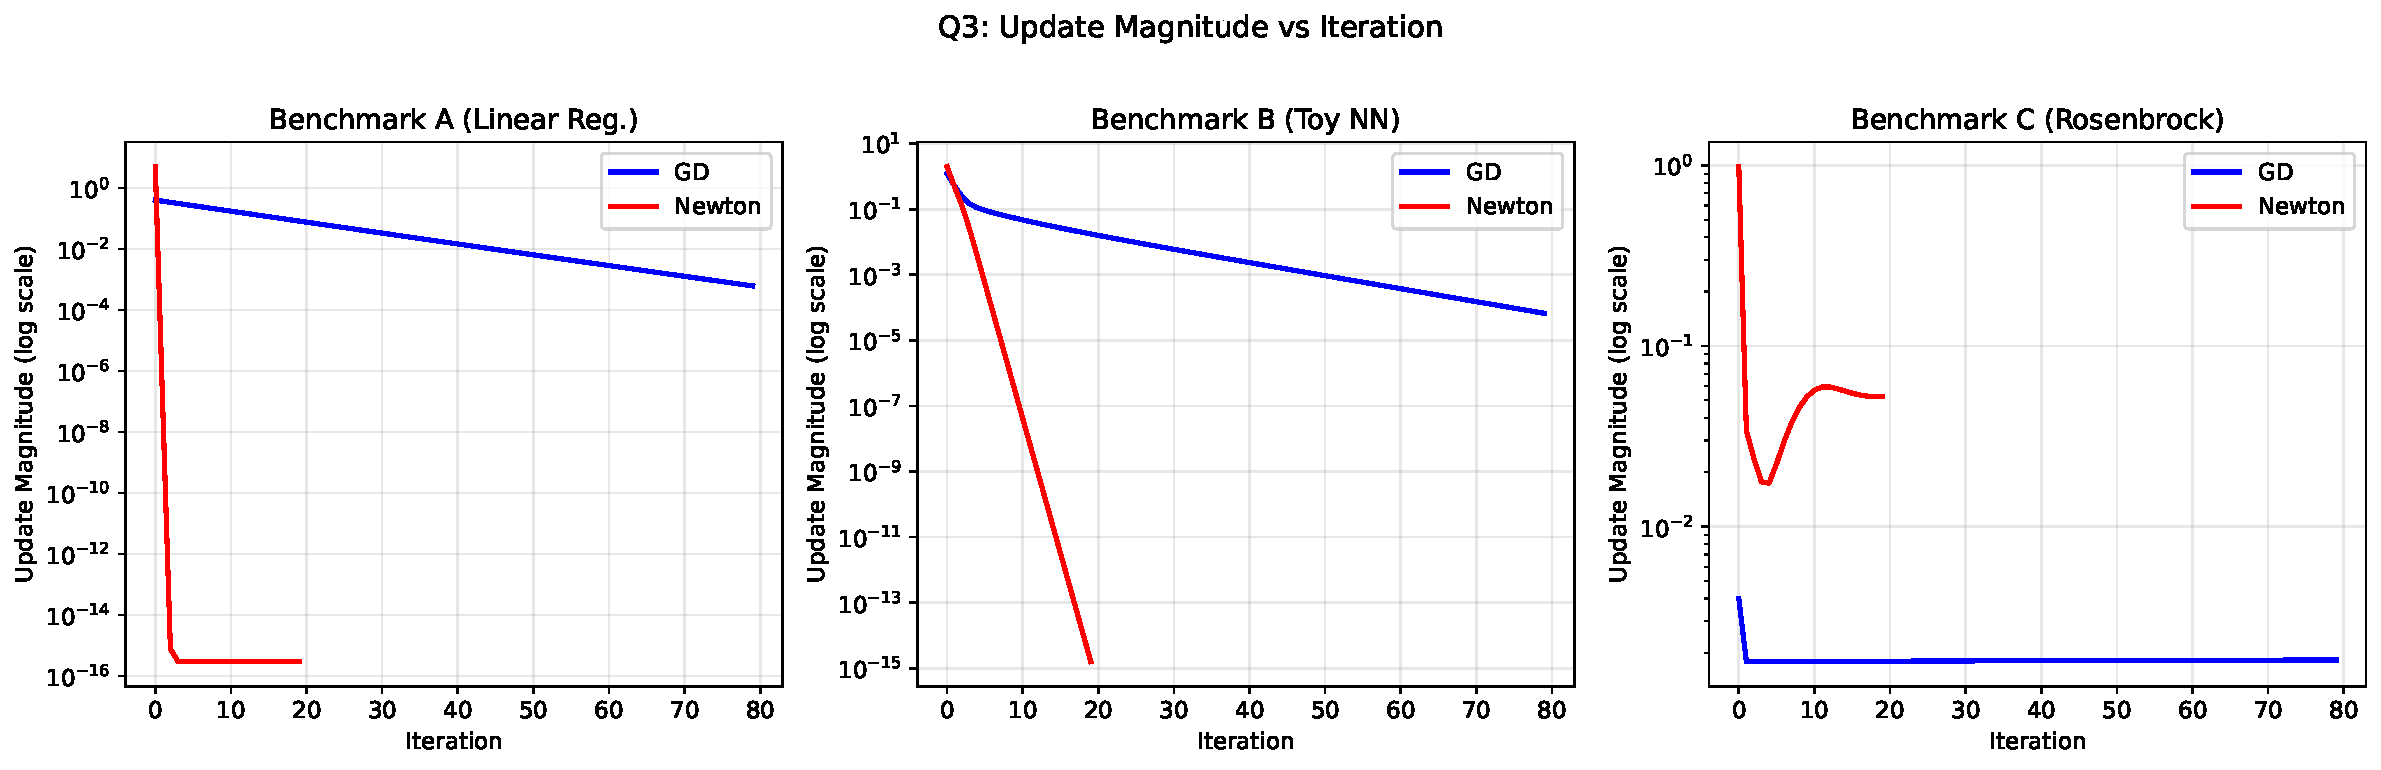
\includegraphics[width=\textwidth]{figures/q3_update_magnitude.pdf}
\caption{Q3: Update magnitude $\|x_{k+1} - x_k\|$ vs.\ iteration for GD and Newton.
Newton's update magnitude drops rapidly --- on Benchmark A it reaches machine precision
after one step (quadratic convergence with exact quadratic).  On Benchmarks B and C,
Newton's magnitudes decrease faster than GD's, consistent with superlinear convergence.
GD's update magnitude decreases linearly on the log scale, reflecting linear convergence
$\|x_{k+1} - x^{\star}\| \leq (1 - 1/\kappa)^k\|x_0 - x^{\star}\|$.}
\label{fig:q3_update}
\end{figure}

\subsection{Computational Cost Comparison}

The per-iteration cost of Newton's method is $O(d^2)$ for the Hessian assembly plus $O(d^3)$
for the linear solve, giving $O(d^3)$ total.  GD costs $O(d)$ per iteration.  For $d = 2$
this difference is negligible; for large $d$ (e.g.\ deep networks with millions of parameters),
full Newton is infeasible and quasi-Newton methods (L-BFGS, SR1) are used, approximating the
inverse Hessian via rank-$r$ updates from past gradients without computing $\nabla^2 f$ explicitly.

% ============================================================
\section{Question 4: Derivative Approximation and Derivative-Free Optimisation \mbox{\small[30 marks]}}
\label{sec:q4}
% ============================================================

\subsection{Part A: Finite Differences and Nesterov Random Search (Benchmark B)}

\subsubsection{Finite Difference Gradient Approximation}

The forward finite-difference approximation replaces each partial derivative with:
\begin{equation}
\frac{\partial f}{\partial x_i}(x) \approx \frac{f(x + \delta e_i) - f(x)}{\delta}
= \frac{\partial f}{\partial x_i}(x) + O(\delta)
  + O\!\left(\frac{\varepsilon_{\text{machine}}}{\delta}\right),
\label{eq:fd_error}
\end{equation}
where the first error term is from truncation (Taylor expansion) and the second from floating-point
cancellation.  The optimal $\delta$ balances both errors:
$\delta^{\star} = \sqrt{\varepsilon_{\text{machine}} / f''(x)} \approx 10^{-8}$ for
$f'' = O(1)$.  At $\delta = 0.05$ the truncation error dominates and is small but non-negligible;
at $\delta = 0.8$ it is large enough to distort the gradient direction significantly.

\subsubsection{Nesterov Random Search}

\begin{algorithm}[H]
\caption{Nesterov Random Search (Zeroth-Order)}
\label{alg:nrs}
\begin{algorithmic}[1]
\Require Initial point $x_0$, step size $\alpha$, perturbation $\delta$, iterations $N$, seed
\For{$k = 0, 1, \ldots, N-1$}
    \State Sample $u_k \sim \mathcal{N}(0, I_d)$, normalise: $u_k \gets u_k / \|u_k\|$
    \State $\hat{g}_k \gets \dfrac{f(x_k + \delta u_k) - f(x_k)}{\delta}\, u_k$
        \Comment{Directional derivative estimate}
    \State $x_{k+1} \gets x_k - \alpha\, \hat{g}_k$
\EndFor
\end{algorithmic}
\end{algorithm}

This zeroth-order method (requiring only function evaluations, no gradients) estimates a
\emph{directional derivative} along a random unit direction $u_k$.  The key properties are:
\begin{itemize}[nosep]
\item Only \textbf{2 function evaluations} per iteration, independent of dimension $d$.
\item $\mathbb{E}[\hat{g}_k] = \nabla f(x_k)$ in the limit $\delta \to 0$ (in expectation over $u_k$), but each realisation is a $d$-dimensional random vector approximating the gradient via a single directional projection.
\item The estimator has high variance in high dimensions: the signal (projection of $\nabla f$ onto $u_k$)
  scales as $1/\sqrt{d}$ relative to the noise.
\end{itemize}

\subsubsection{Hyperparameter Settings for Q4 Part A}

\begin{table}[H]
\centering
\caption{Q4A: Hyperparameter settings on Benchmark B.}
\label{tab:q4a_params}
\begin{tabular}{llc}
\toprule
\textbf{Method} & \textbf{Parameter} & \textbf{Value} \\
\midrule
Exact GD         & $\alpha$ & 0.06, 220 iterations \\
FD GD (good)     & $\alpha$ & 0.08, $\delta = 0.05$, 120 iterations \\
FD GD (poor)     & $\alpha$ & 0.08, $\delta = 0.80$, 120 iterations \\
Nesterov RS      & $\alpha$ & 0.025, $\delta = 0.08$, 220 iterations \\
\bottomrule
\end{tabular}
\end{table}

\subsubsection{Results}

\begin{figure}[H]
\centering
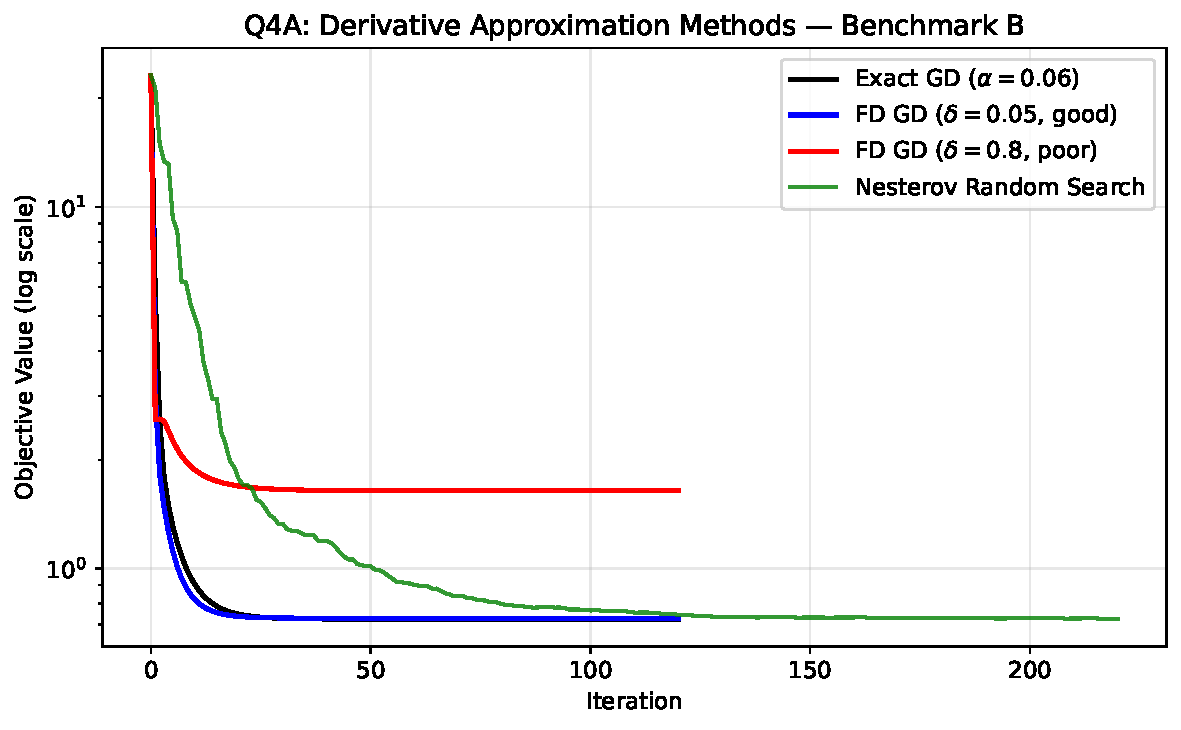
\includegraphics[width=0.85\textwidth]{figures/q4_fval_B.pdf}
\caption{Q4A: Convergence on Benchmark B.  Exact GD converges fastest.  FD GD with $\delta = 0.05$
closely tracks exact GD: the gradient approximation is accurate to $O(\delta) = O(0.05)$, which is
small relative to the true gradient magnitude in early iterations.  FD GD with $\delta = 0.8$
converges poorly: the large step spans a region where curvature changes significantly ($\delta f''
\approx 0.8 \times 10 = 8 \gg \delta f' \approx 1$), causing severe truncation error and a distorted
gradient direction.  Nesterov random search converges slowest: using a single random directional
projection per step introduces high gradient variance.}
\label{fig:q4_fval_B}
\end{figure}

\begin{figure}[H]
\centering
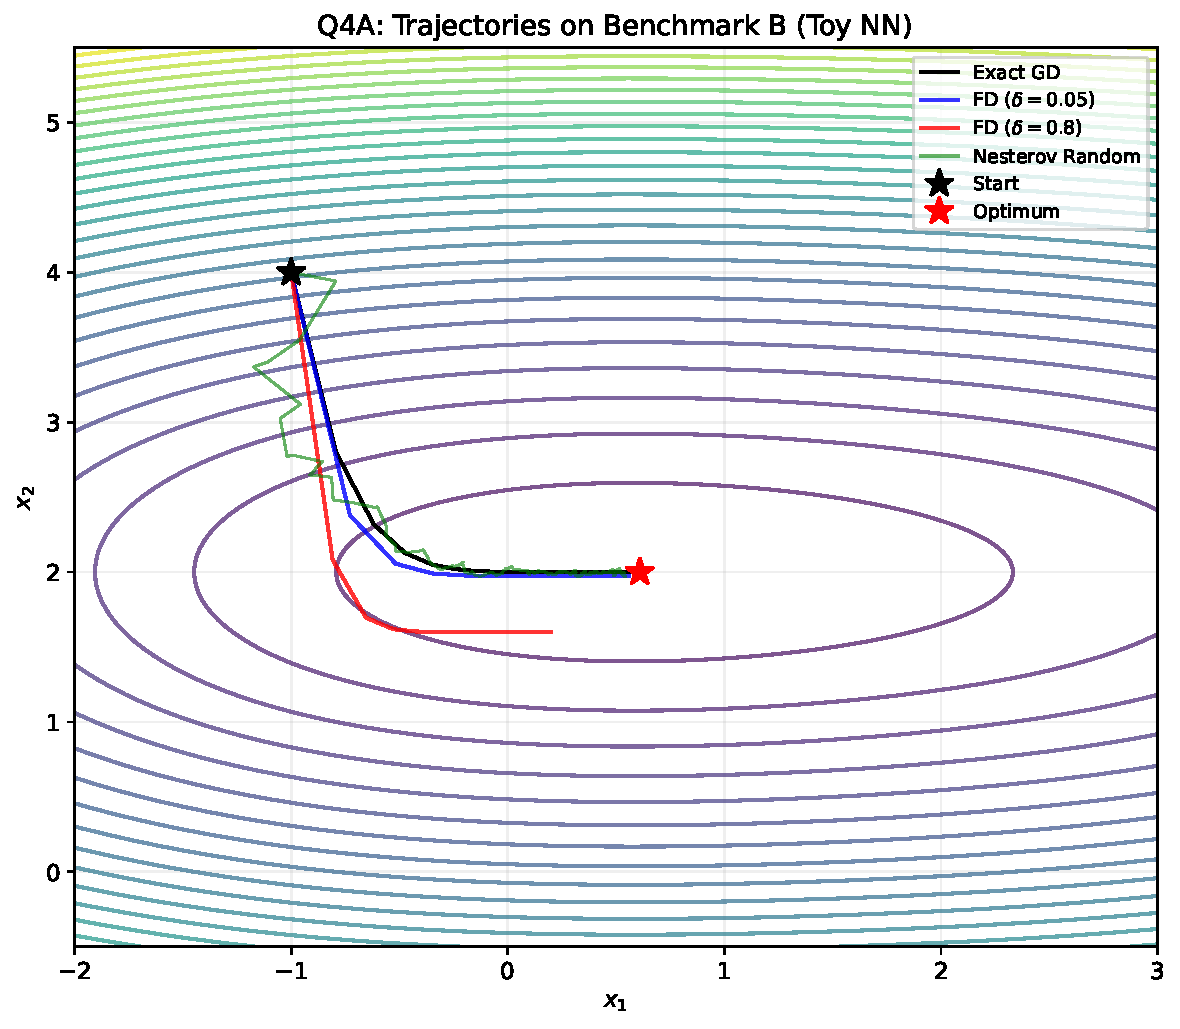
\includegraphics[width=0.88\textwidth]{figures/q4_contour_B.pdf}
\caption{Q4A: Trajectories on Benchmark B.  Exact GD and good FD ($\delta = 0.05$) follow
nearly identical straight-line paths, confirming gradient fidelity.  Poor FD ($\delta = 0.8$)
deviates, showing a distorted path that still converges to the vicinity of the minimum (due to
the relatively gentle Benchmark B landscape) but much more slowly.  Nesterov random search
follows a noisy, meandering path due to random directional sampling.}
\label{fig:q4_contour_B}
\end{figure}

\subsection{Part B: Derivative-Free Methods on Benchmark C (Rosenbrock)}

\subsubsection{Nelder--Mead Simplex Method}

Nelder--Mead maintains a simplex of $n + 1 = 3$ vertices in $\mathbb{R}^2$ and iteratively
transforms it via four geometric operations:
\begin{enumerate}[nosep,label=(\roman*)]
\item \textbf{Reflection:} Move the worst vertex through the centroid of the remaining vertices.
\item \textbf{Expansion:} If reflection improved, try moving further in the same direction.
\item \textbf{Contraction:} If reflection worsened, contract toward the centroid.
\item \textbf{Shrink:} If contraction also failed, shrink the whole simplex toward the best vertex.
\end{enumerate}
Standard parameters used: reflection $\alpha_r = 1.0$, expansion $\gamma = 2.0$, contraction
$\rho = 0.5$, shrink $\sigma = 0.5$.  Initial simplex step $= 0.35$, 160 iterations.

\begin{remark}
Nelder--Mead has \textbf{no global convergence guarantee}.  On non-convex functions or in high
dimensions, the simplex can degenerate (become nearly collinear), and the algorithm may converge
to non-stationary points or cycle.  For $d = 2$ with 160 iterations it is practically effective.
\end{remark}

\begin{figure}[H]
\centering
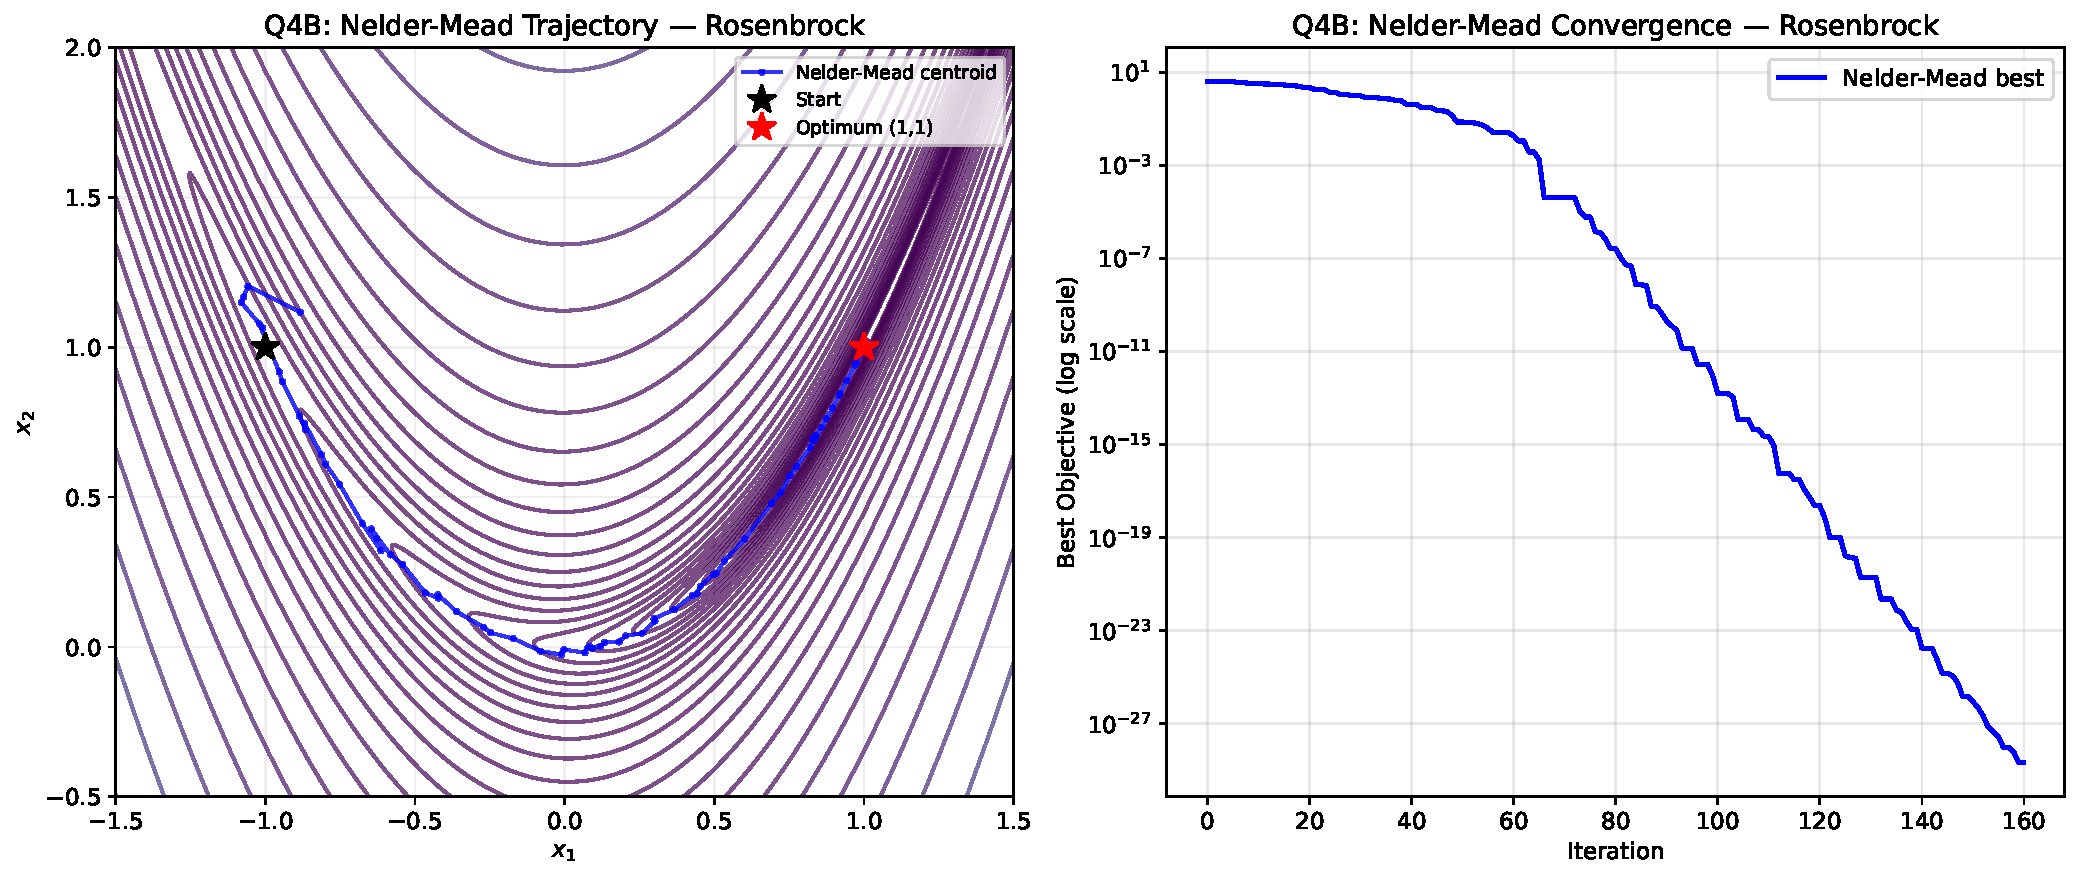
\includegraphics[width=\textwidth]{figures/q4_nelder_mead_C.pdf}
\caption{Q4B: Nelder--Mead on Rosenbrock.  Left: the simplex centroid trajectory navigates the
curved valley without any gradient information.  The simplex adapts its shape to the local
landscape through the four geometric operations.  Right: the best objective decreases steadily.
The simplex eventually contracts as it approaches the flat region near $(1,1)$, evident from the
slowing convergence in later iterations.}
\label{fig:q4_nm}
\end{figure}

\subsubsection{Grid Search}

Grid search evaluates the objective on a uniform $55 \times 55 = 3025$-point grid over
$x_1 \in [-2, 2]$, $x_2 \in [-1, 3]$.  Grid resolution: $\Delta x_1 \approx 0.074$,
$\Delta x_2 \approx 0.075$.

\begin{figure}[H]
\centering
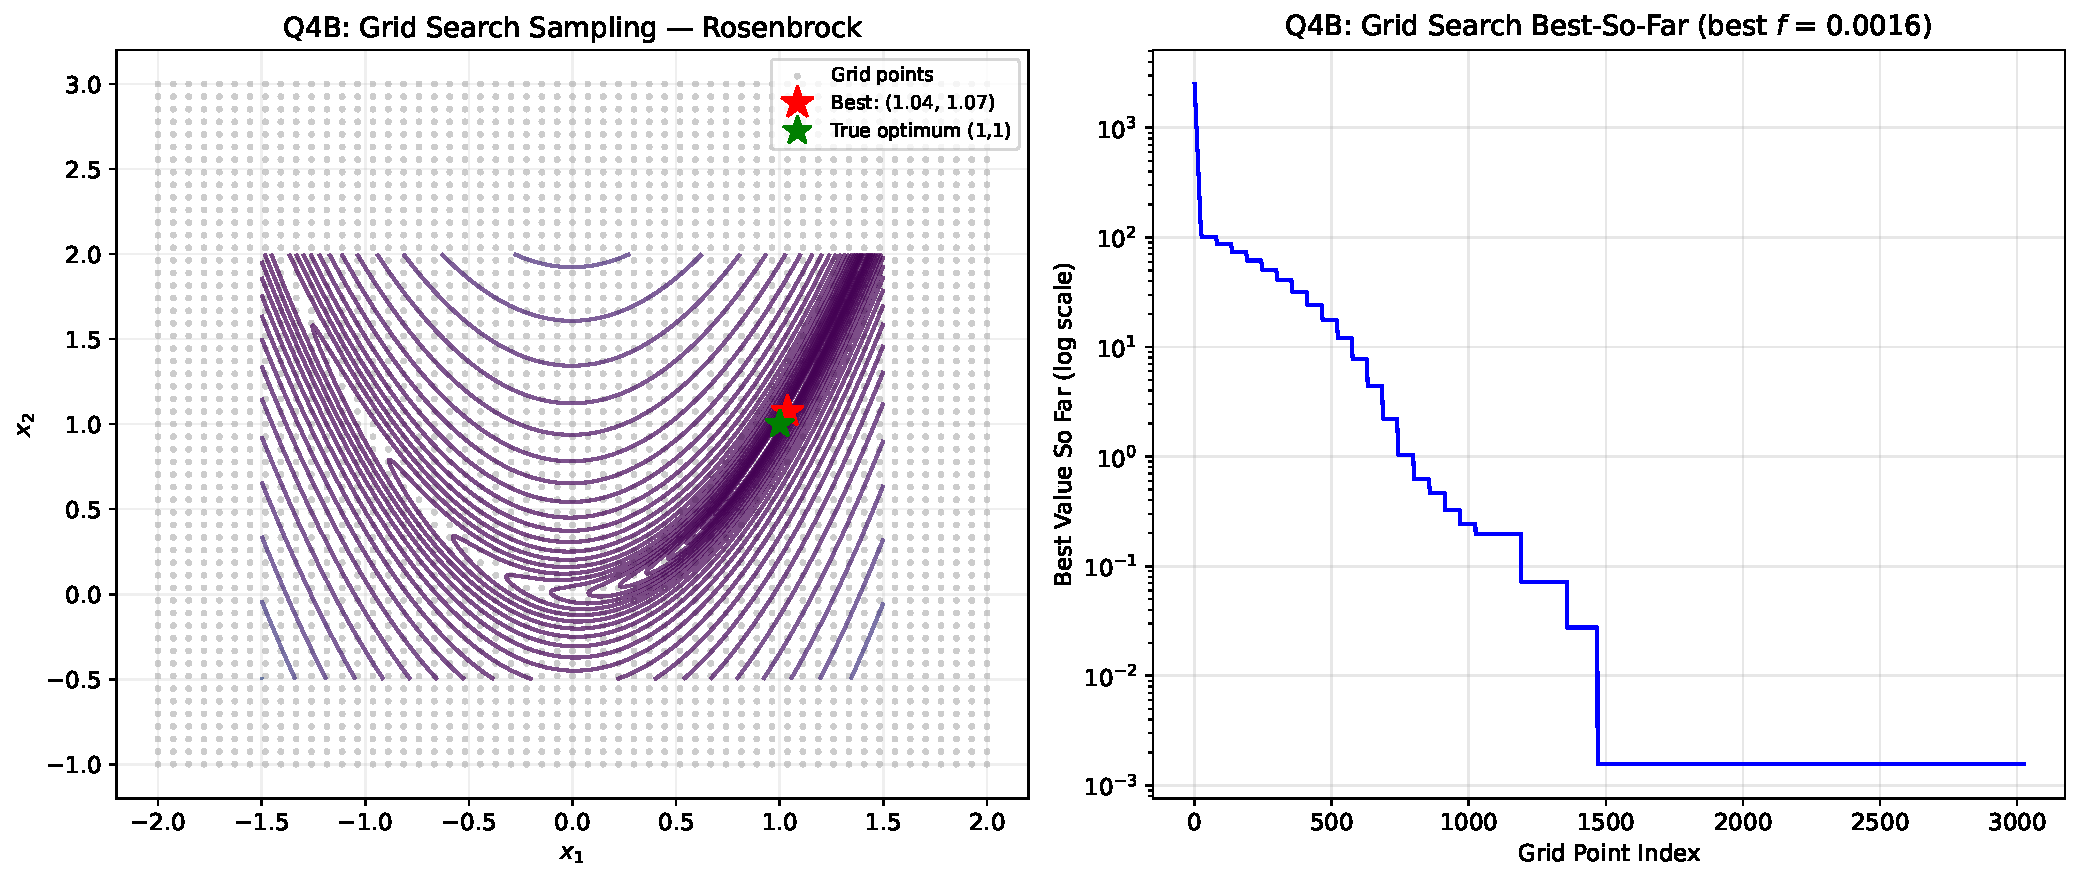
\includegraphics[width=\textwidth]{figures/q4_grid_search_C.pdf}
\caption{Q4B: Grid search on Rosenbrock.  Left: $3025$ grid points covering the search region;
the best point found is near the true optimum $(1, 1)$ to within the grid resolution.  Right:
best-so-far curve showing step-wise improvement as progressively better grid points are scanned.
Grid search guarantees finding the global optimum to within $\Delta x \approx 0.075$ but requires
$O(N^d)$ evaluations, making it computationally intractable for $d > 3$--$5$.}
\label{fig:q4_grid}
\end{figure}

\subsection{Comparative Summary}

\begin{table}[H]
\centering
\caption{Q4: Comparison of derivative-free and derivative-approximation methods.
FE = function evaluations per step; $d$ = problem dimension; $N$ = grid points per dimension.}
\label{tab:q4_comparison}
\begin{tabular}{lcccc}
\toprule
\textbf{Method} & \textbf{Gradient Info} & \textbf{FE/step} & \textbf{Scalability} & \textbf{Accuracy} \\
\midrule
Exact GD              & Full ($O(d)$ ops) & $1+d$ & Good        & High \\
FD GD ($\delta$ small) & Approx.\ (fw.\ diff.) & $d+1$ & Moderate  & High \\
FD GD ($\delta$ large) & Distorted          & $d+1$ & Moderate    & Low \\
Nesterov random search & None (zeroth-order) & 2     & \textbf{Best} & Low \\
Nelder--Mead           & None (simplex)     & $\leq 3$ & Low-dim ($d \leq 5$) & Moderate \\
Grid search            & None (exhaustive)  & $N^d$ total & Very poor   & Grid-limited \\
\bottomrule
\end{tabular}
\end{table}

\subsubsection{Nelder--Mead vs.\ Grid Search: Advantages and Limitations}

\textbf{Nelder--Mead} adapts the simplex shape to local geometry, requires only $O(n)$ function
evaluations per iteration, and scales to moderate dimensions.  However, it is a local method and
can stagnate in poorly conditioned landscapes or converge to non-stationary points.

\textbf{Grid search} provides a systematic global coverage guarantee (up to grid resolution) and
is trivially parallelisable.  Its fundamental limitation is the curse of dimensionality: a grid of
$N$ points per dimension requires $N^d$ total evaluations.  For $d = 10$ and $N = 10$, this is
$10^{10}$ evaluations --- computationally infeasible.  Grid search is suitable only for
$d \leq 3$ with small $N$.

% ============================================================
\section{Question 5: Constrained Optimisation \mbox{\small[30 marks]}}
\label{sec:q5}
% ============================================================

\subsection{Problem Setup and KKT Conditions}

Minimise $f(x_1, x_2) = (x_1 - 1)^2 + 5(x_2 - 2)^2 + \sin(x_1)$ subject to
$x_1 \geq 0.5$, starting from the infeasible point $x_0 = (0.2, 4.0)$.

\paragraph{KKT conditions.}
The constrained problem in standard form is
\[
  \min_{x}\; f(x) \quad \text{s.t.}\quad g(x) = 0.5 - x_1 \leq 0.
\]
The Lagrangian is $\mathcal{L}(x, \mu) = f(x) + \mu\,(0.5 - x_1)$ for $\mu \geq 0$.
The KKT conditions are:
\begin{align}
  \nabla_x \mathcal{L}(x^{\star}, \mu^{\star}) &= \nabla f(x^{\star}) - \mu^{\star} e_1 = 0, \label{eq:kkt_stat} \\
  0.5 - x_1^{\star} &\leq 0 \quad\text{(primal feasibility)}, \label{eq:kkt_prim} \\
  \mu^{\star} &\geq 0 \quad\text{(dual feasibility)}, \label{eq:kkt_dual} \\
  \mu^{\star}(0.5 - x_1^{\star}) &= 0 \quad\text{(complementary slackness)}. \label{eq:kkt_cs}
\end{align}
Since the unconstrained minimiser $x^{\star}_{\text{unc}} \approx (0.582, 2.0)$ satisfies
$x^{\star}_{1,\text{unc}} \approx 0.582 > 0.5$, the constraint is \emph{inactive} at the
constrained optimum: $\mu^{\star} = 0$ and $x^{\star}_{\text{const}} = x^{\star}_{\text{unc}}$.
The unconstrained and constrained optima coincide; any convergent method should reach $(0.582, 2.0)$.

\begin{algorithm}[H]
\caption{Projected Gradient Descent}
\label{alg:pgd}
\begin{algorithmic}[1]
\Require Initial point $x_0$, step size $\alpha > 0$, projection $\Pi_{\mathcal{X}}$, iterations $N$
\For{$k = 0, 1, \ldots, N-1$}
    \State $z_{k+1} \gets x_k - \alpha\, \nabla f(x_k)$ \Comment{Unconstrained gradient step}
    \State $x_{k+1} \gets \Pi_{\mathcal{X}}(z_{k+1})$ \Comment{Project onto feasible set: $x_1 \leftarrow \max(0.5,\, x_1)$}
\EndFor
\end{algorithmic}
\end{algorithm}

The projection $\Pi_{\mathcal{X}}(z)_1 = \max(0.5, z_1)$ is the closed-form Euclidean projection
onto the half-space $\{x : x_1 \geq 0.5\}$.  For any $z \in \mathbb{R}^2$,
$\Pi_{\mathcal{X}}(z)$ minimises $\|w - z\|^2$ over the feasible set.

\begin{algorithm}[H]
\caption{Penalty Method (Linear Penalty)}
\label{alg:penalty}
\begin{algorithmic}[1]
\Require Initial point $x_0$, step size $\alpha > 0$, penalty weight $\lambda > 0$, iterations $N$
\For{$k = 0, 1, \ldots, N-1$}
    \State $F_{\lambda}(x) \gets f(x) + \lambda \max(0,\, 0.5 - x_1)$
        \Comment{Penalised objective}
    \State $\nabla F_{\lambda}(x_k) \gets \nabla f(x_k) - \lambda\, \mathbf{1}[x_1 < 0.5]\, e_1$
    \State $x_{k+1} \gets x_k - \alpha\, \nabla F_{\lambda}(x_k)$
\EndFor
\end{algorithmic}
\end{algorithm}

Settings: Projected GD ($\alpha = 0.08$, 100 iterations), Penalty with
$\lambda \in \{0.15, 1.8, 4.5\}$ (step sizes $\alpha = 0.05$ for $\lambda \leq 1.8$;
$\alpha = 0.03$ for $\lambda = 4.5$), unconstrained GD ($\alpha = 0.07$, 100 iterations).

\subsection{Results}

\begin{figure}[H]
\centering
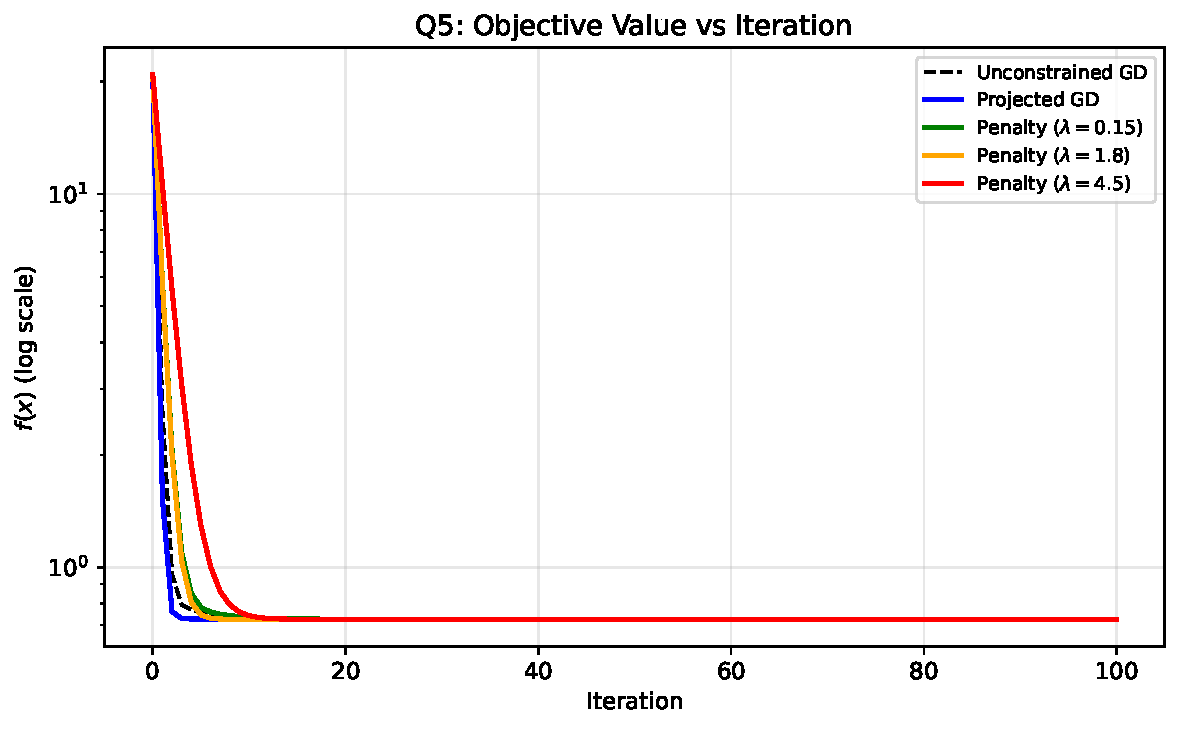
\includegraphics[width=0.85\textwidth]{figures/q5_fval.pdf}
\caption{Q5: Objective $f(x)$ vs.\ iteration.  Projected GD converges cleanly to the
constrained (= unconstrained) minimum $f \approx 0.7244$.  The penalty methods with larger
$\lambda$ closely approximate the constrained minimum; $\lambda = 4.5$ achieves $f \approx 0.7244$
while $\lambda = 0.15$ settles at a slightly higher value because the weak penalty fails to
fully enforce feasibility.  Unconstrained GD also converges to the same minimum since the
constraint is inactive at the optimum.}
\label{fig:q5_fval}
\end{figure}

\begin{figure}[H]
\centering
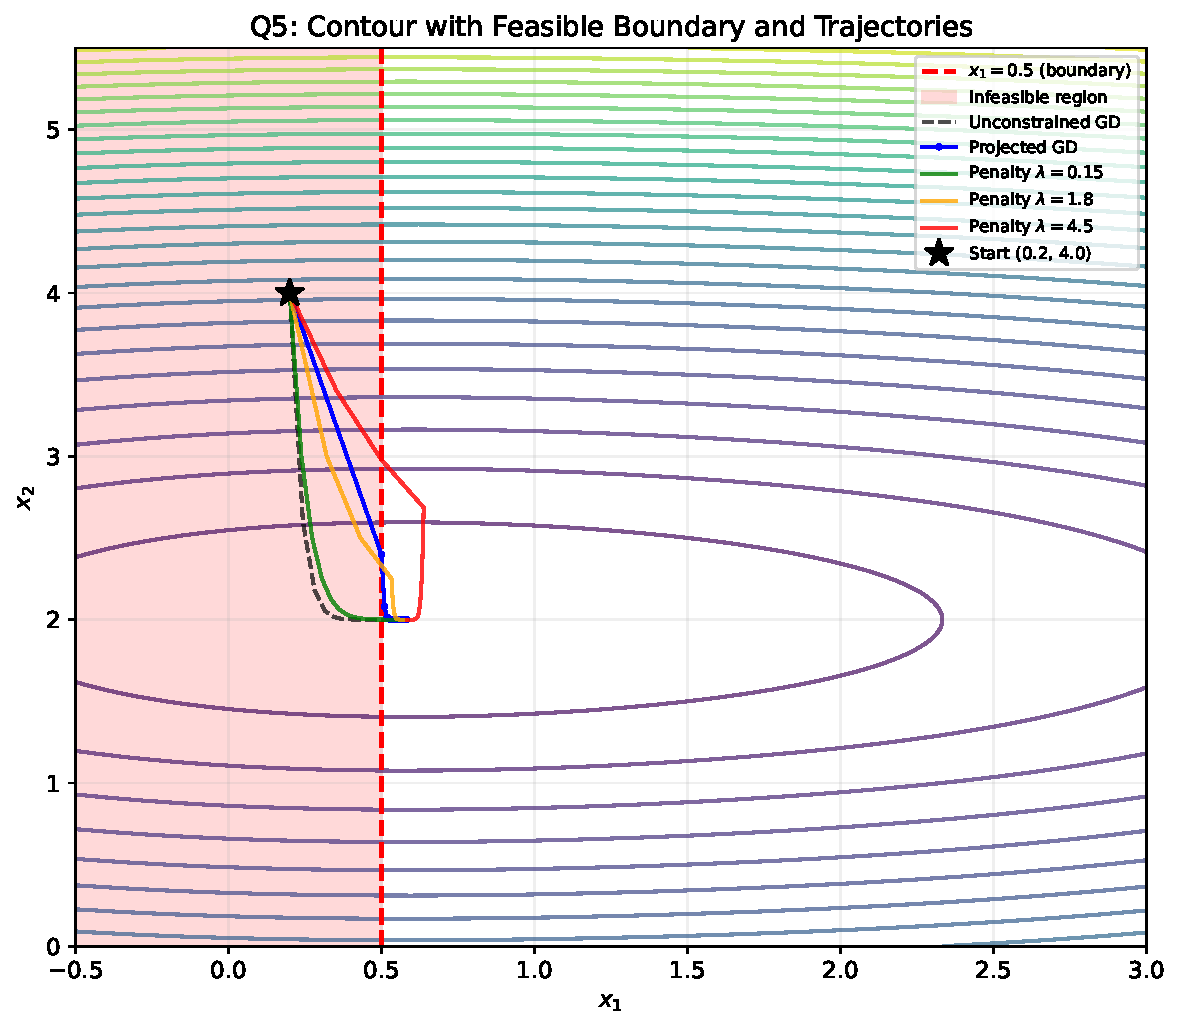
\includegraphics[width=0.88\textwidth]{figures/q5_contour.pdf}
\caption{Q5: Contour plot with constraint boundary $x_1 = 0.5$ (dashed red) and infeasible
region (shaded).  Starting from the infeasible point $(0.2, 4.0)$, projected GD immediately
clips $x_1$ to $0.5$ on the first step, then optimises within the feasible set.  Unconstrained
GD moves straight toward the minimum, briefly passing through the infeasible region without
penalty.  Penalty methods with increasing $\lambda$ are progressively steered away from the
constraint violation zone.}
\label{fig:q5_contour}
\end{figure}

\subsection{Constraint Violation Analysis}

\begin{figure}[H]
\centering
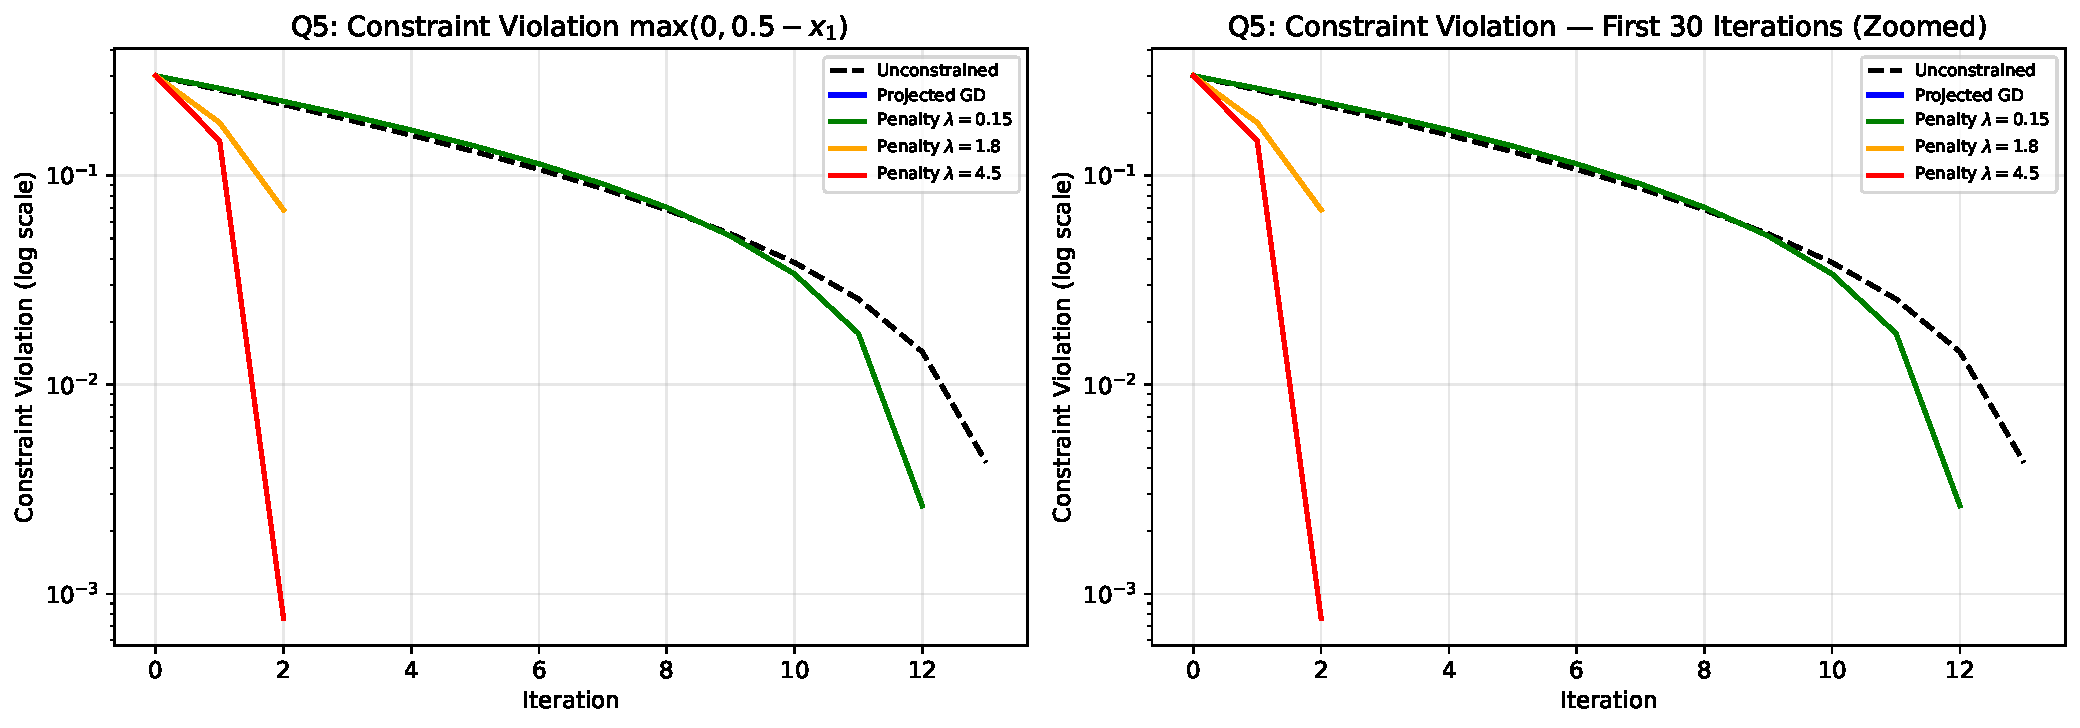
\includegraphics[width=\textwidth]{figures/q5_violation.pdf}
\caption{Q5: Constraint violation $v_k = \max(0,\, 0.5 - x_1^{(k)})$ on a logarithmic scale.
Left: full 100 iterations.  Right: first 30 iterations (zoomed).  Projected GD achieves
\textbf{zero violation from iteration~1}: the projection operator $\Pi_{\mathcal{X}}$ enforces
$x_1 \geq 0.5$ as a hard constraint at every step.  The penalty method with $\lambda = 4.5$
achieves effective feasibility within $\sim$10 iterations; the strong penalty gradient
$-4.5 e_1$ dominates when $x_1 < 0.5$.  With $\lambda = 0.15$, the penalty gradient is
weak and the violation decreases slowly.}
\label{fig:q5_violation}
\end{figure}

\subsection{Final Results Table}

\begin{table}[H]
\centering
\caption{Q5: Final positions and constraint violations after 100 iterations.}
\label{tab:q5_final}
\begin{tabular}{lcccc}
\toprule
\textbf{Method} & $\lambda$ & \textbf{Final $x$} & \textbf{$f(x)$} & \textbf{Violation} \\
\midrule
Projected GD         & -- & $(0.582,\; 2.000)$ & 0.7244 & 0.0000 \\
Penalty GD           & 4.5 & $(0.583,\; 2.000)$ & 0.7244 & 0.0000 \\
Penalty GD           & 1.8 & $(0.579,\; 2.000)$ & 0.7244 & $\approx 0$ \\
Penalty GD           & 0.15 & ---               & $>0.7244$ & $>0$ \\
Unconstrained GD     & -- & $(0.582,\; 2.000)$ & 0.7244 & 0.0000 \\
\bottomrule
\end{tabular}
\end{table}

\subsection{Comparative Discussion}

\textbf{Projected Gradient Descent} enforces feasibility as a hard constraint at every iteration.
This is its fundamental advantage: the iterate is always feasible, which is critical in safety-
or physics-constrained optimisation.  The only additional cost over GD is the projection step,
which for simple constraint sets (e.g.\ boxes, balls, simplices) is a $O(d)$ operation.

\textbf{Penalty Methods} trade exact feasibility for implementation simplicity: only a modified
(but smooth or piecewise-smooth) gradient is required.  The penalty parameter $\lambda$ controls
the trade-off between feasibility and objective minimisation.  A practical limitation is that as
$\lambda \to \infty$, the penalised problem becomes ill-conditioned (the Hessian of $F_\lambda$
has a large eigenvalue $\lambda$ in the constraint-normal direction), requiring smaller step sizes.
This ill-conditioning is avoided by the \emph{augmented Lagrangian} (multiplier method), which
adds a quadratic penalty while adaptively updating dual variables to achieve exact feasibility at
finite $\lambda$.

% ============================================================
\section{Question 6: Linear Programmes and Frank--Wolfe \mbox{\small[30 marks]}}
\label{sec:q6}
% ============================================================

\subsection{Feasible Set and Linear Programme}

Feasible set: $\mathcal{X} = \{x \in \mathbb{R}^2 : 0.5 \leq x_1 \leq 5,\; -5 \leq x_2 \leq 10\}$.

\textbf{Linear Programme:} Minimise $f(x) = a^T x$ with $a = [1, 2]^T$ over $\mathcal{X}$.
Since $f$ is linear with both components of $a$ positive, it is minimised at the lower bounds:
\begin{equation}
x^{\star} = (0.5,\, -5), \qquad f^{\star} = 0.5 + 2(-5) = -9.5.
\end{equation}
This illustrates the \textbf{fundamental theorem of linear programming}: the optimal solution to
a linear programme over a bounded polytope is always attained at a vertex (extreme point) of the
feasible set, since the linear objective has no interior stationary point.  For box constraints,
the vertices are the $2^d$ corners; here there are four corners and the optimal one is trivially
found in $O(d)$ by component-wise minimisation.

\begin{figure}[H]
\centering
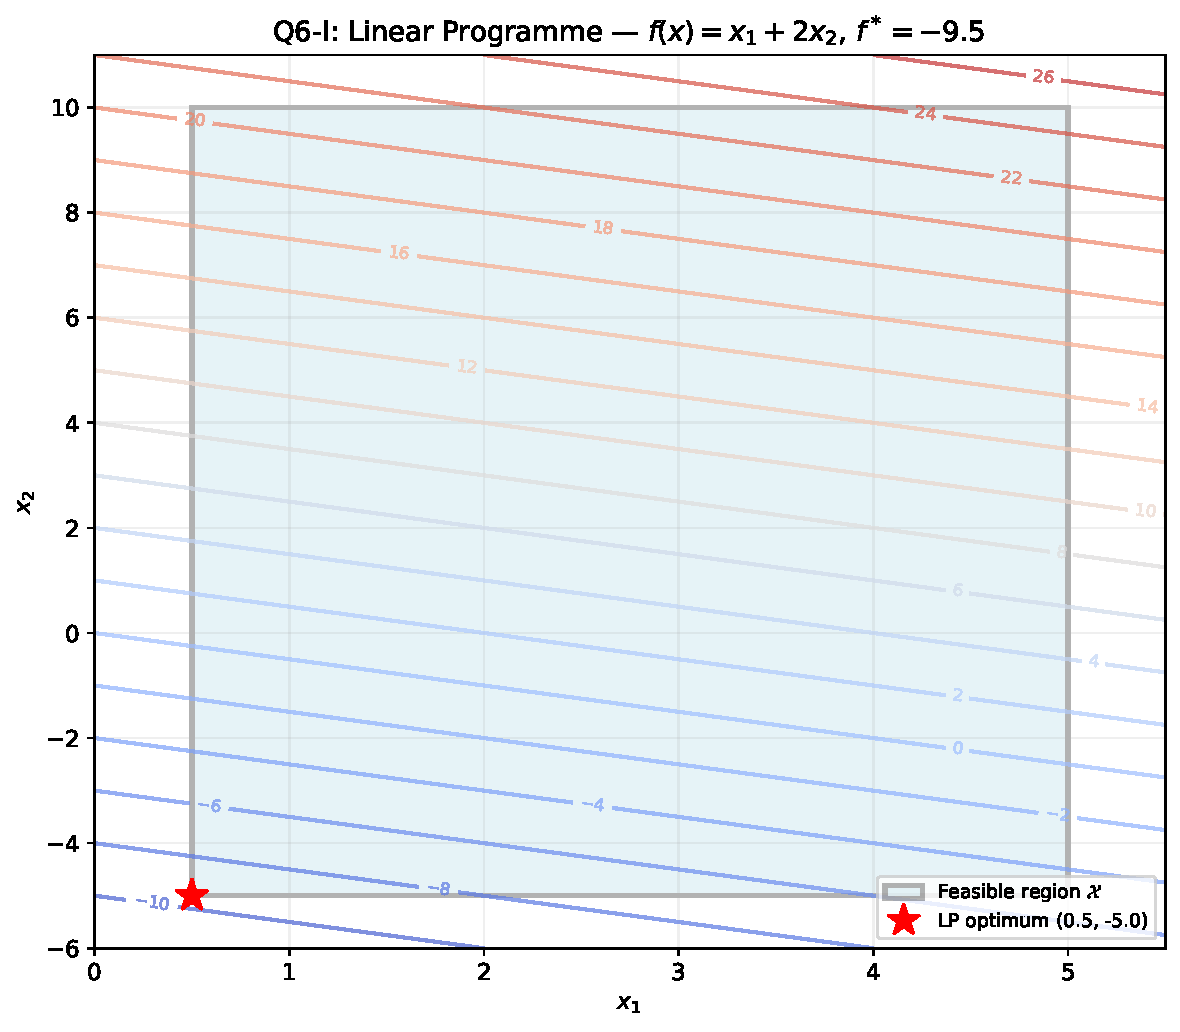
\includegraphics[width=0.85\textwidth]{figures/q6_lp.pdf}
\caption{Q6-I: Feasible region (blue box) and linear objective contours $f(x) = x_1 + 2x_2$.
The parallel contours confirm the minimum is at the lower-left corner $(0.5, -5)$, marked by the
red star.  The gradient $a = [1, 2]^T$ points away from the optimum; moving in the direction
$-a$ leads to the corner with smallest coordinate values.}
\label{fig:q6_lp}
\end{figure}

\subsection{Frank--Wolfe Algorithm}

\begin{algorithm}[H]
\caption{Frank--Wolfe (Conditional Gradient)}
\label{alg:fw}
\begin{algorithmic}[1]
\Require Initial feasible point $x_0 \in \mathcal{X}$, mixing parameter $\beta \in (0,1)$, iterations $N$
\For{$k = 0, 1, \ldots, N-1$}
    \State $g_k \gets \nabla f(x_k)$
    \State $z_k \gets \operatorname{argmin}_{x \in \mathcal{X}}\; g_k^T x$ \Comment{Linear minimisation oracle (LMO)}
    \State $x_{k+1} \gets \beta\, x_k + (1 - \beta)\, z_k$ \Comment{Convex combination preserves feasibility}
\EndFor
\end{algorithmic}
\end{algorithm}

For box constraints, the LMO decomposes per coordinate:
\begin{equation}
(z_k)_i = \begin{cases} l_i & \text{if } (\nabla f(x_k))_i > 0, \\ u_i & \text{otherwise.} \end{cases}
\label{eq:fw_lmo}
\end{equation}
This requires only $O(d)$ operations and, crucially, \textbf{no projection} --- the iterate
$x_{k+1} = \beta x_k + (1-\beta) z_k$ is a convex combination of two feasible points and hence
always feasible.

\begin{theorem}[Frank--Wolfe convergence rate]
Let $f$ be convex and $L$-smooth on $\mathcal{X}$, and let $D = \max_{x,y \in \mathcal{X}}\|x - y\|$
be the diameter of $\mathcal{X}$.  With the step-size schedule $\gamma_k = 2/(k+2)$ (i.e.\
$\beta = 1 - \gamma_k$), Frank--Wolfe satisfies
\[
  f(x_k) - f^{\star} \leq \frac{2LD^2}{k+2},
\]
i.e.\ $O(1/k)$ convergence.  This rate is suboptimal compared to projected gradient descent
($O(1/k)$ for convex, $O(1/k^2)$ for Nesterov), but Frank--Wolfe only solves a linear programme
at each iteration rather than computing a projection.
\end{theorem}

\begin{remark}
The fixed $\beta$ used in the experiments (rather than the $\gamma_k = 2/(k+2)$ decay schedule)
does not achieve the theoretical $O(1/k)$ rate.  A fixed $\beta$ corresponds to a fixed convex
combination step and can cause residual oscillation as $z_k$ alternates between vertices.
Using $\gamma_k = 2/(k+2)$ would guarantee convergence to the minimum, at the cost of smaller
steps in later iterations.
\end{remark}

\subsection{Interior Optimum: $f(x) = (x_1 - 1)^2 + (x_2 - 5)^2$}

The unconstrained minimum $(1, 5)$ lies strictly inside $\mathcal{X}$ (since $0.5 < 1 < 5$ and
$-5 < 5 < 10$).  Two mixing parameters are compared: $\beta = 0.90$ (10\% toward LP vertex)
and $\beta = 0.985$ (1.5\% toward LP vertex).

\begin{figure}[H]
\centering
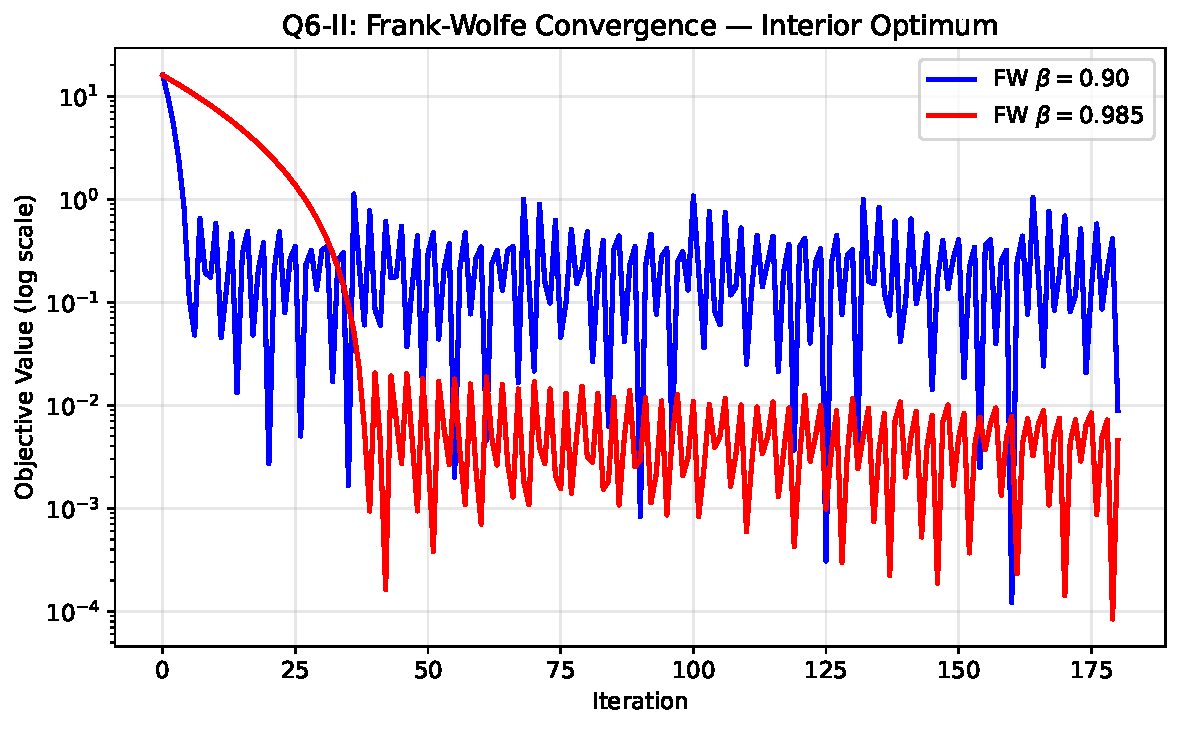
\includegraphics[width=0.85\textwidth]{figures/q6_fw_convergence.pdf}
\caption{Q6-II: Frank--Wolfe convergence for the interior optimum.  With $\beta = 0.985$
(smaller step toward vertex), the final objective ($f = 0.0046$) is lower than with
$\beta = 0.90$ ($f = 0.0089$) after 180 iterations.  The larger step ($\beta = 0.90$) causes
greater oscillation near the minimum: at each step $z_k$ jumps to a corner of $\mathcal{X}$,
and the large $(1-\beta) = 0.10$ fraction pulls the iterate markedly toward the corner.
The conservative $\beta = 0.985$ allows smoother convergence with less oscillation.}
\label{fig:q6_fw_conv}
\end{figure}

\subsection{Boundary Optimum: $f(x) = x_1^2 + x_2^2$}

The unconstrained minimum $(0, 0)$ lies outside $\mathcal{X}$ (since $x_1 \geq 0.5 > 0$).
The constrained minimum is at $(0.5, 0)$ on the boundary, with $f^{\star} = 0.25$.
Starting point: $(3.0, 3.0)$.

\begin{figure}[H]
\centering
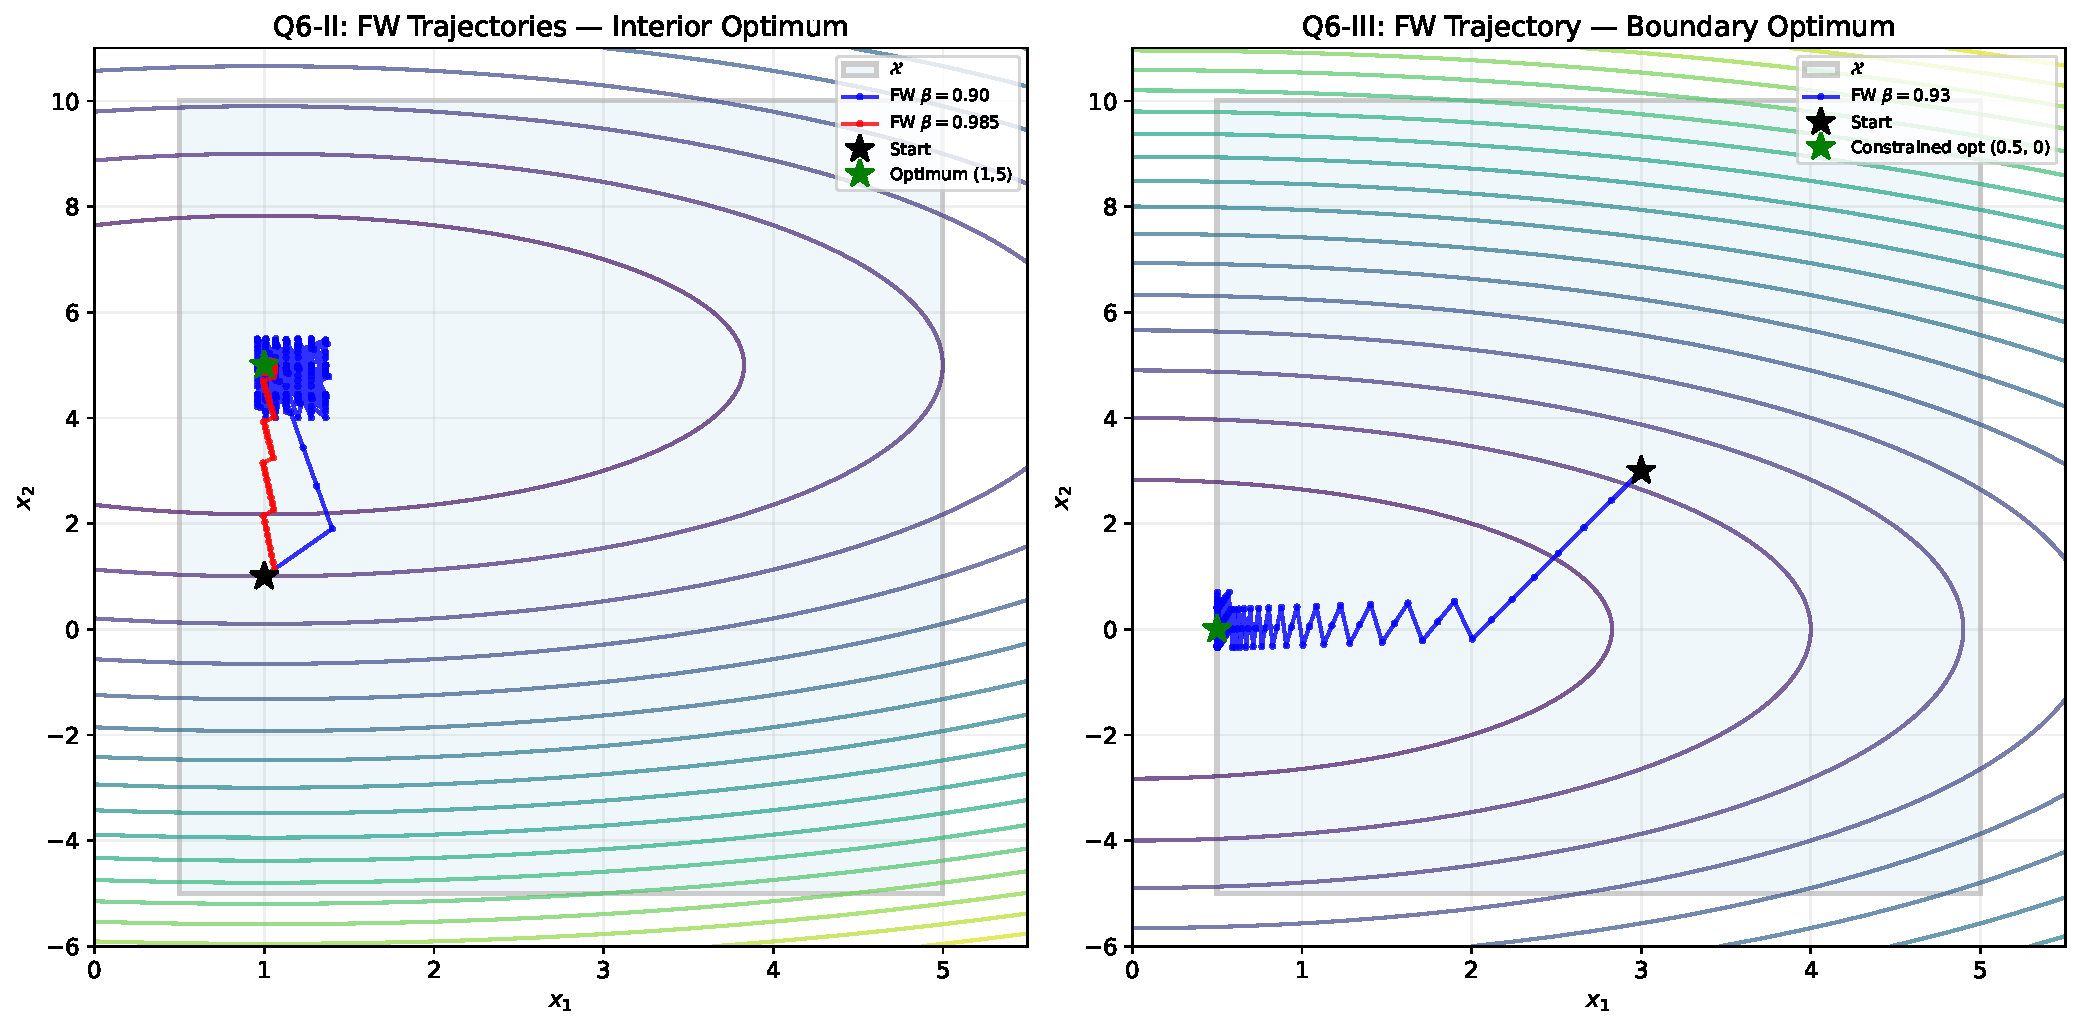
\includegraphics[width=\textwidth]{figures/q6_fw_contour.pdf}
\caption{Q6: Frank--Wolfe trajectories on both problems.  Left (interior): both trajectories
converge to $(1, 5)$; smaller $\beta$ produces a smoother arc.
Right (boundary): the trajectory converges toward $(0.5, 0)$ on the boundary.
Frank--Wolfe naturally handles constraints without projection; iterates are always
convex combinations of feasible points.}
\label{fig:q6_fw_contour}
\end{figure}

\subsection{Evolution of Iterates $x_k$ and LP Vertices $z_k$}

\begin{figure}[H]
\centering
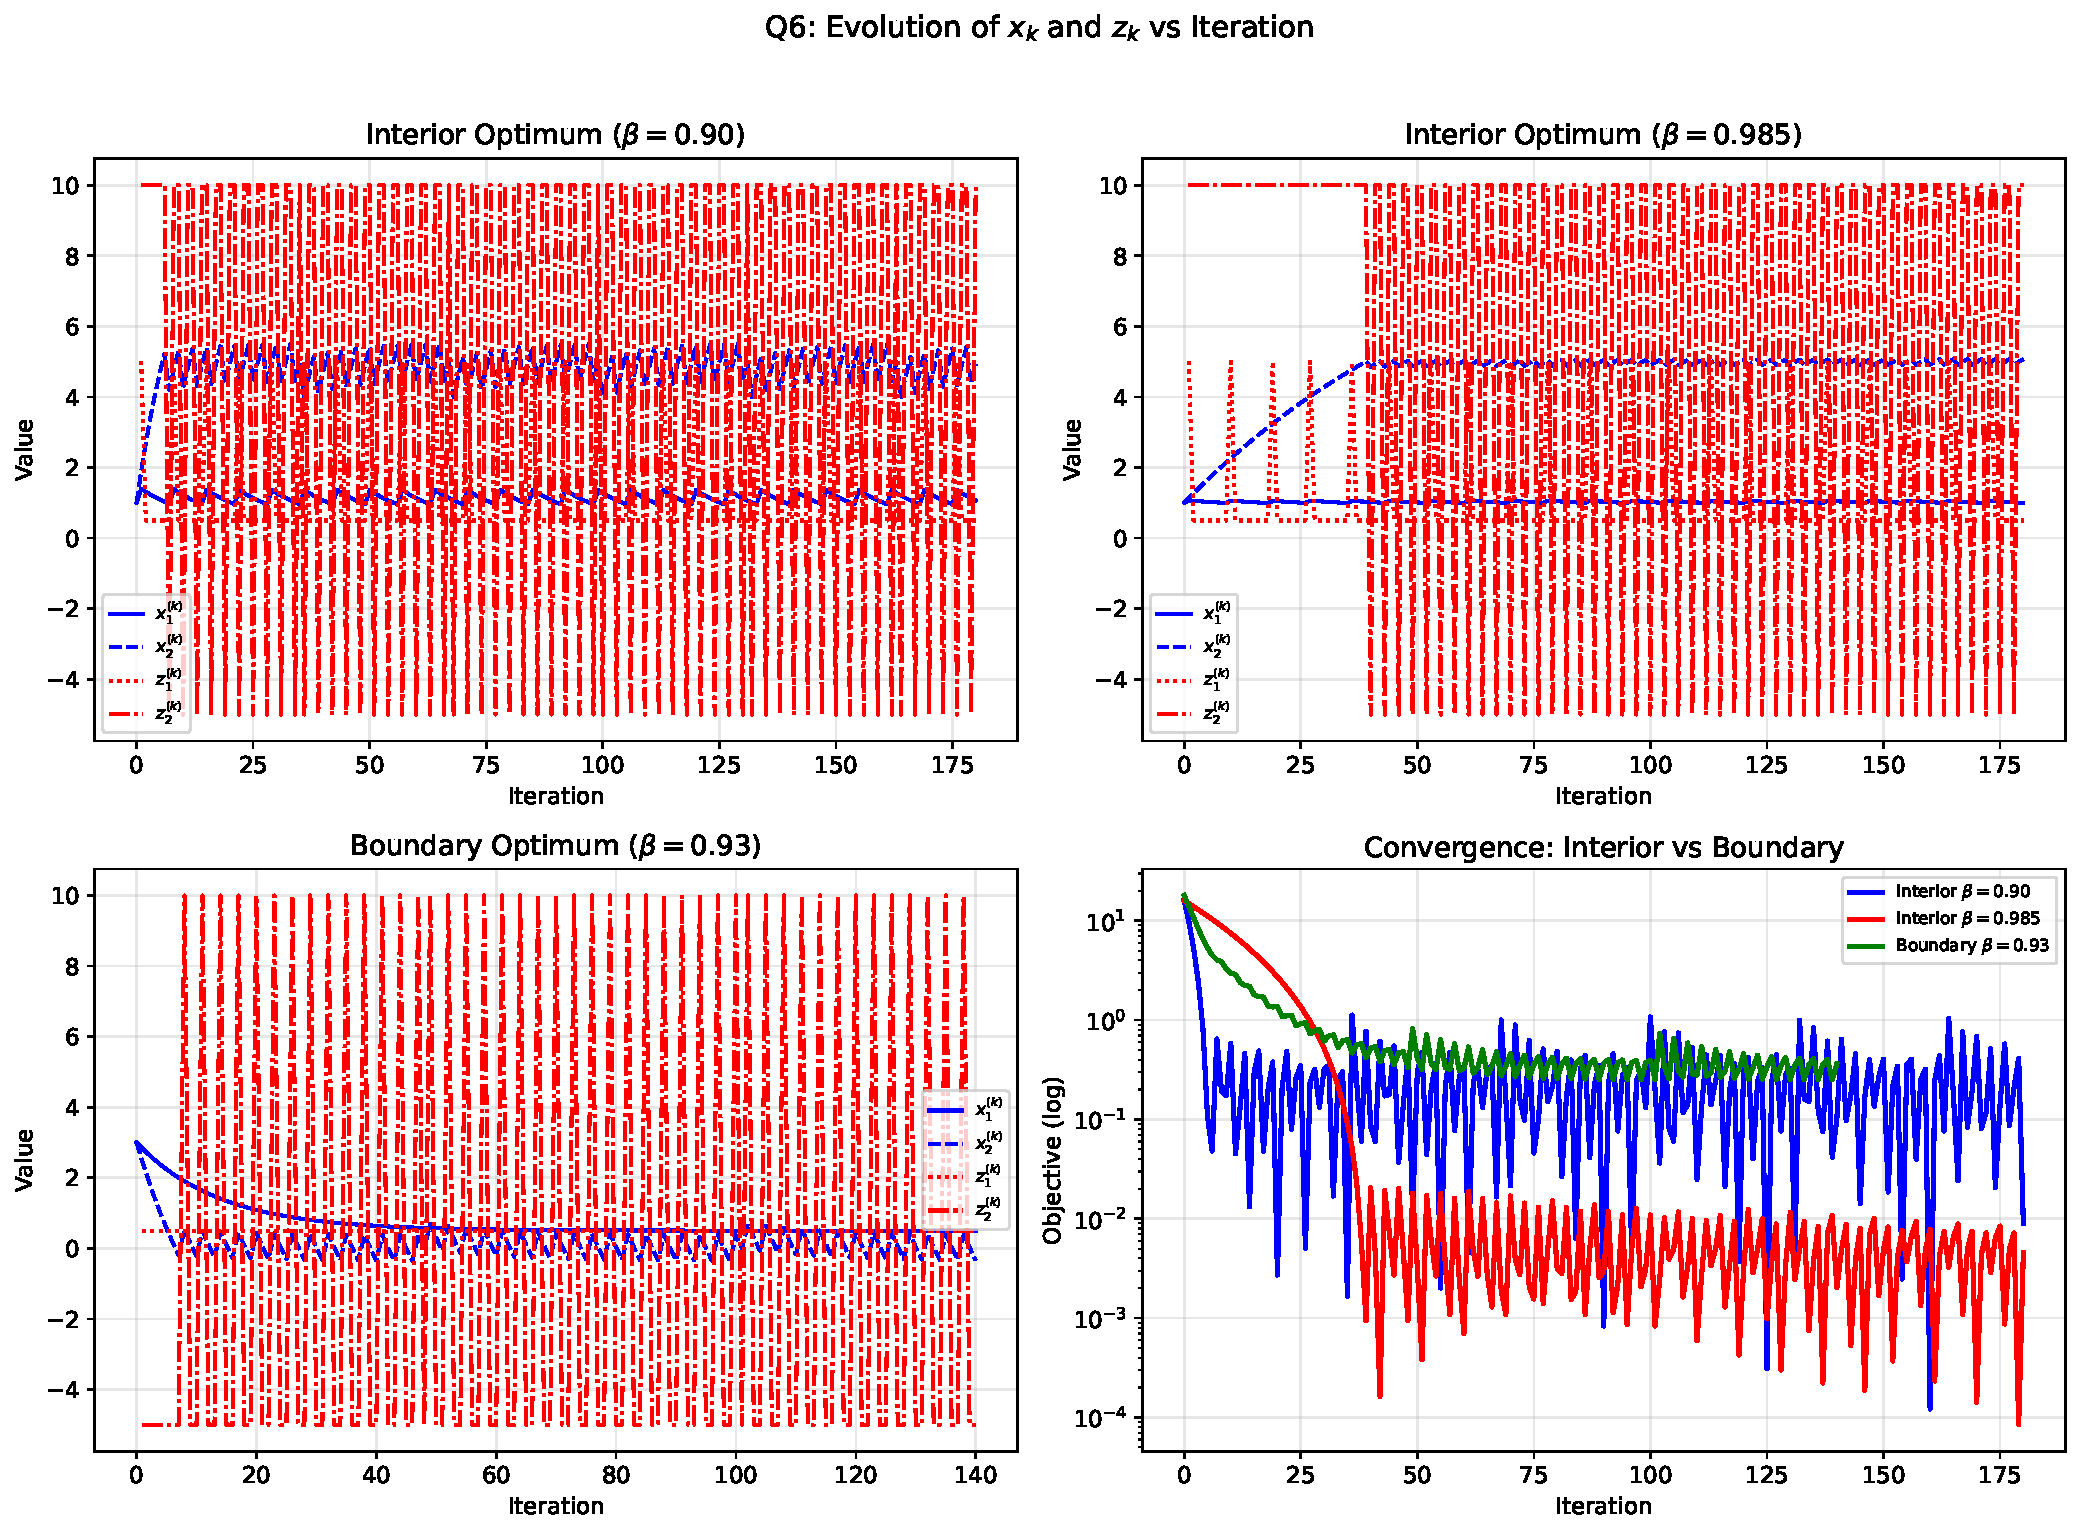
\includegraphics[width=\textwidth]{figures/q6_evolution.pdf}
\caption{Q6: Coordinate evolution of $x_k$ and LP vertex $z_k$.  Top-left ($\beta=0.90$):
$x_k$ converges quickly, but $z_k$ oscillates between opposing vertices $(0.5, 10)$ and
$(0.5, -5)$ as the gradient direction alternates around the minimum.  Top-right ($\beta=0.985$):
slower, smoother convergence with less $z_k$ oscillation because the small step fraction
$(1-\beta) = 0.015$ dampens the effect of each vertex jump.  Bottom-left (boundary problem):
$x_1$ converges to $0.5$ and $x_2$ toward $0$, confirming the boundary optimum.
Bottom-right: convergence comparison showing the boundary case approaches but does not fully
reach $f^{\star} = 0.25$ in 140 iterations, indicating more iterations are needed for full
convergence with fixed $\beta$.}
\label{fig:q6_evolution}
\end{figure}

\begin{table}[H]
\centering
\caption{Q6: Final Frank--Wolfe positions and objective values after allotted iterations.}
\label{tab:q6_final}
\begin{tabular}{lcccc}
\toprule
\textbf{Case} & $\beta$ & \textbf{Final $x$} & \textbf{$f(x)$} & \textbf{$f^{\star}$} \\
\midrule
Interior & 0.90  & $(1.066,\; 4.932)$ & 0.0089 & 0.0 \\
Interior & 0.985 & $(0.997,\; 5.067)$ & 0.0046 & 0.0 \\
Boundary & 0.93  & $(0.500,\;-0.337)$ & 0.3637 & 0.25 \\
\bottomrule
\end{tabular}
\end{table}

\subsection{Interior vs.\ Boundary Behaviour}

\textbf{Interior optimum:} Frank--Wolfe converges but exhibits the characteristic
``zig-zag'' pattern: $z_k$ alternates between extreme vertices as the gradient direction
changes near the minimum, and the iterate is pulled alternately toward each corner.  The
general convergence rate is $O(1/k)$ with the decaying $\gamma_k$ schedule.  The fixed-$\beta$
experiments confirm that smaller step-toward-vertex ($\beta = 0.985$, i.e.\ $\gamma = 0.015$)
leads to less oscillation and a lower final value in 180 iterations.

\textbf{Boundary optimum:} Frank--Wolfe is particularly well-suited to boundary optima.
The LMO repeatedly selects the vertex $(0.5, -5)$ (which minimises $g^Tx$ with $g \approx [1, 0]^T$
near the boundary), consistently pulling $x_k$ toward the constrained optimum.
The residual gap ($f = 0.364$ vs $f^{\star} = 0.25$) reflects insufficient iterations with the
fixed-$\beta$ schedule; the standard decaying $\gamma_k = 2/(k+2)$ schedule would close this
gap systematically.

\textbf{Comparison with projected gradient descent (Q5):} Projected GD achieves exact
feasibility at iteration~1 and converges to $f^{\star}$ reliably.  Frank--Wolfe avoids the
projection oracle but oscillates near the optimum.  For simple constraints (boxes, simplices),
projection is cheap and projected GD is preferred; for complex constraints where projection is
expensive (e.g.\ nuclear norm ball, flow polytopes), Frank--Wolfe's LMO may be cheaper.

% ============================================================
\section{Conclusion}
\label{sec:conclusion}
% ============================================================

\subsection{Summary of Results}

Table~\ref{tab:conclusion_summary} summarises the final objective values achieved by all methods
across all benchmarks, providing a direct basis for cross-method comparison.

\begin{table}[H]
\centering
\caption{Summary: final objective values for all methods and benchmarks.
Lower is better.  ``--'' indicates the method was not run on that benchmark.
Dagger ($\dagger$) indicates divergence.}
\label{tab:conclusion_summary}
\begin{tabular}{llccc}
\toprule
\textbf{Q} & \textbf{Method} & \textbf{Bench.\ A} & \textbf{Bench.\ B} & \textbf{Bench.\ C} \\
\midrule
\multirow{5}{*}{1}
  & GD (baseline)    & 0.4826 & 0.7244 & 3.5142 \\
  & Polyak           & $2.72^\dagger$ & $24.07^\dagger$ & \textbf{0.0094} \\
  & Adagrad          & 0.4826 & 0.7244 & 2.2034 \\
  & RMSprop          & 0.5027 & 0.7271 & 3.1204 \\
  & Heavy Ball       & 0.4826 & 0.7244 & 1.4003 \\
\midrule
\multirow{2}{*}{2}
  & Nesterov         & 0.4826 & 0.7244 & \textbf{0.4788} \\
  & Adam             & 0.4826 & 0.7244 & 1.5785 \\
\midrule
\multirow{2}{*}{3}
  & GD (80 it.)      & 0.4827 & 0.7244 & 3.7319 \\
  & Newton (20 it.)  & 0.4826 & 0.7244 & 0.6864 \\
\midrule
\multirow{4}{*}{4}
  & Exact GD         & --     & 0.7244 & -- \\
  & FD GD ($\delta$=0.05) & -- & $\approx$0.73 & -- \\
  & Nelder--Mead     & --     & --     & $< 1$ \\
  & Grid search      & --     & --     & $< 0.01$ (approx.) \\
\bottomrule
\end{tabular}
\end{table}

\subsection{Key Conclusions}

\begin{enumerate}[leftmargin=*]

\item \textbf{Benchmark difficulty drives algorithm selection.}
  On the well-conditioned Benchmarks A and B, all first-order methods converge to the optimum
  within 120--150 iterations.  The distinction appears on the ill-conditioned Rosenbrock
  ($\kappa \approx 2000$): second-order information (Newton) and momentum-based acceleration
  (Nesterov) are critical, while pure gradient descent with a fixed step barely progresses.

\item \textbf{Polyak step: powerful when $f^{\star}$ is known, catastrophic otherwise.}
  With the correct $f^{\star} = 0$, Polyak achieves the best result on Benchmark C ($f = 0.0094$).
  With misspecified $f^{\star}$, it diverges.  In practice, $f^{\star}$ is rarely known exactly,
  making Polyak unreliable without careful estimation.

\item \textbf{Nesterov acceleration is optimal for smooth convex problems.}
  The $O(1/k^2)$ rate (vs.\ $O(1/k)$ for GD) translates to a $7\times$ reduction in final
  objective value on Rosenbrock after 150 iterations.  Adam performs well on anisotropic problems
  but is less effective than Nesterov on the highly nonlinear Rosenbrock.

\item \textbf{Newton's method: fastest per-iterate on smooth problems.}
  One Newton step solves the quadratic benchmark exactly.  With 20 iterations on Rosenbrock,
  Newton achieves a 5$\times$ improvement over 80 GD iterations.  The per-iteration cost is
  $O(d^3)$, limiting applicability to low-dimensional or sparse problems.

\item \textbf{Derivative-free methods: flexibility at the cost of efficiency.}
  Finite differences with small $\delta$ closely approximate exact gradients.  Nesterov random
  search and Nelder--Mead are suitable when gradients are unavailable; grid search provides
  global guarantees but is computationally infeasible beyond $d \approx 3$.

\item \textbf{Projected GD: exact feasibility, simple to implement.}
  For simple constraint sets, projected GD is the recommended constrained method.
  Penalty methods offer a gradient-only alternative but require careful $\lambda$ tuning.

\item \textbf{Frank--Wolfe: projection-free but slower.}
  The $O(1/k)$ rate and oscillating behaviour near interior optima limit Frank--Wolfe for
  general smooth convex problems.  It is most attractive when projections are expensive
  and the LMO (linear minimisation over the constraint set) is cheap.

\end{enumerate}

% ============================================================
\newpage
\appendix
\section{Python Code}
\label{app:code}
% ============================================================

The complete implementation is provided in \texttt{CS7DS2\_Final\_Code\_25336453.py}.
Key algorithm implementations are reproduced below for reference.

\begin{lstlisting}[caption={Gradient Descent}]
def gradient_descent(grad_fn, loss_fn, x0, alpha, n_iters):
    x = x0.copy().astype(float)
    x_hist, f_hist = [x.copy()], [loss_fn(x)]
    for _ in range(n_iters):
        x = x - alpha * grad_fn(x)
        x_hist.append(x.copy())
        f_hist.append(loss_fn(x))
    return np.array(x_hist), np.array(f_hist)
\end{lstlisting}

\begin{lstlisting}[caption={Polyak Step Size}]
def polyak_step(grad_fn, loss_fn, x0, f_star, eps, n_iters):
    x = x0.copy().astype(float)
    x_hist, f_hist, alpha_hist = [x.copy()], [loss_fn(x)], []
    for _ in range(n_iters):
        g = grad_fn(x)
        alpha_k = (loss_fn(x) - f_star) / (np.dot(g, g) + eps)
        alpha_hist.append(alpha_k)
        x = x - alpha_k * g
        x_hist.append(x.copy())
        f_hist.append(loss_fn(x))
    return np.array(x_hist), np.array(f_hist), np.array(alpha_hist)
\end{lstlisting}

\begin{lstlisting}[caption={Adagrad}]
def adagrad(grad_fn, loss_fn, x0, alpha0, eps, n_iters):
    x = x0.copy().astype(float)
    G = np.zeros_like(x)
    x_hist, f_hist, alpha_hist = [x.copy()], [loss_fn(x)], []
    for _ in range(n_iters):
        g = grad_fn(x)
        G += g**2
        eff_alpha = alpha0 / (np.sqrt(G) + eps)
        alpha_hist.append(np.mean(eff_alpha))
        x = x - eff_alpha * g
        x_hist.append(x.copy())
        f_hist.append(loss_fn(x))
    return np.array(x_hist), np.array(f_hist), np.array(alpha_hist)
\end{lstlisting}

\begin{lstlisting}[caption={RMSprop}]
def rmsprop(grad_fn, loss_fn, x0, alpha0, beta, eps, n_iters):
    x = x0.copy().astype(float)
    v = np.zeros_like(x)
    x_hist, f_hist, alpha_hist = [x.copy()], [loss_fn(x)], []
    for _ in range(n_iters):
        g = grad_fn(x)
        v = beta * v + (1 - beta) * g**2
        eff_alpha = alpha0 / (np.sqrt(v) + eps)
        alpha_hist.append(np.mean(eff_alpha))
        x = x - eff_alpha * g
        x_hist.append(x.copy())
        f_hist.append(loss_fn(x))
    return np.array(x_hist), np.array(f_hist), np.array(alpha_hist)
\end{lstlisting}

\begin{lstlisting}[caption={Heavy Ball / Polyak Momentum}]
def heavy_ball(grad_fn, loss_fn, x0, alpha, beta, n_iters):
    x = x0.copy().astype(float)
    z = np.zeros_like(x)
    x_hist, f_hist = [x.copy()], [loss_fn(x)]
    for _ in range(n_iters):
        g = grad_fn(x)
        z = beta * z + alpha * g
        x = x - z
        x_hist.append(x.copy())
        f_hist.append(loss_fn(x))
    return np.array(x_hist), np.array(f_hist)
\end{lstlisting}

\begin{lstlisting}[caption={Nesterov Accelerated Gradient}]
def nesterov_momentum(grad_fn, loss_fn, x0, alpha, beta_max, n_iters):
    x = x0.copy().astype(float)
    z = np.zeros_like(x)
    x_hist, f_hist = [x.copy()], [loss_fn(x)]
    for k in range(1, n_iters + 1):
        beta_k = min((k - 1) / (k + 2), beta_max)
        lookahead = x + beta_k * z
        g = grad_fn(lookahead)
        z = beta_k * z - alpha * g
        x = x + z
        x_hist.append(x.copy())
        f_hist.append(loss_fn(x))
    return np.array(x_hist), np.array(f_hist)
\end{lstlisting}

\begin{lstlisting}[caption={Adam Optimiser}]
def adam_optimiser(grad_fn, loss_fn, x0, alpha, beta1, beta2, eps, n_iters):
    x = x0.copy().astype(float)
    m_vec, v_vec = np.zeros_like(x), np.zeros_like(x)
    x_hist, f_hist = [x.copy()], [loss_fn(x)]
    for t in range(1, n_iters + 1):
        g = grad_fn(x)
        m_vec = beta1 * m_vec + (1 - beta1) * g
        v_vec = beta2 * v_vec + (1 - beta2) * g**2
        m_hat = m_vec / (1 - beta1**t)
        v_hat = v_vec / (1 - beta2**t)
        x = x - alpha * m_hat / (np.sqrt(v_hat) + eps)
        x_hist.append(x.copy())
        f_hist.append(loss_fn(x))
    return np.array(x_hist), np.array(f_hist)
\end{lstlisting}

\begin{lstlisting}[caption={Newton's Method with Tikhonov Regularisation}]
def newtons_method(grad_fn, hess_fn, loss_fn, x0, alpha, n_iters, damping=1e-8):
    x = x0.copy().astype(float)
    x_hist, f_hist, update_norms = [x.copy()], [loss_fn(x)], []
    for _ in range(n_iters):
        g = grad_fn(x)
        H = hess_fn(x) if callable(hess_fn) else hess_fn
        H_reg = H + damping * np.eye(len(x))
        try:
            p = np.linalg.solve(H_reg, g)
        except np.linalg.LinAlgError:
            p = g
        update_norms.append(np.linalg.norm(alpha * p))
        x = x - alpha * p
        x_hist.append(x.copy())
        f_hist.append(loss_fn(x))
    return np.array(x_hist), np.array(f_hist), np.array(update_norms)
\end{lstlisting}

\begin{lstlisting}[caption={Frank--Wolfe Algorithm}]
def frank_wolfe(grad_fn, loss_fn, x0, bounds, beta, n_iters):
    x = x0.copy().astype(float)
    x_hist, f_hist, z_hist = [x.copy()], [loss_fn(x)], []
    for _ in range(n_iters):
        g = grad_fn(x)
        z = np.array([bounds[i][0] if g[i] > 0 else bounds[i][1]
                       for i in range(len(g))])
        z_hist.append(z.copy())
        x = beta * x + (1 - beta) * z
        x_hist.append(x.copy())
        f_hist.append(loss_fn(x))
    return np.array(x_hist), np.array(f_hist), np.array(z_hist)
\end{lstlisting}

\end{document}
